\documentclass[twoside]{book}

% Packages required by doxygen
\usepackage{fixltx2e}
\usepackage{calc}
\usepackage{doxygen}
\usepackage[export]{adjustbox} % also loads graphicx
\usepackage{graphicx}
\usepackage[utf8]{inputenc}
\usepackage{makeidx}
\usepackage{multicol}
\usepackage{multirow}
\PassOptionsToPackage{warn}{textcomp}
\usepackage{textcomp}
\usepackage[nointegrals]{wasysym}
\usepackage[table]{xcolor}

% Font selection
\usepackage[T1]{fontenc}
\usepackage[scaled=.90]{helvet}
\usepackage{courier}
\usepackage{amssymb}
\usepackage{sectsty}
\renewcommand{\familydefault}{\sfdefault}
\allsectionsfont{%
  \fontseries{bc}\selectfont%
  \color{darkgray}%
}
\renewcommand{\DoxyLabelFont}{%
  \fontseries{bc}\selectfont%
  \color{darkgray}%
}
\newcommand{\+}{\discretionary{\mbox{\scriptsize$\hookleftarrow$}}{}{}}

% Page & text layout
\usepackage{geometry}
\geometry{%
  a4paper,%
  top=2.5cm,%
  bottom=2.5cm,%
  left=2.5cm,%
  right=2.5cm%
}
\tolerance=750
\hfuzz=15pt
\hbadness=750
\setlength{\emergencystretch}{15pt}
\setlength{\parindent}{0cm}
\setlength{\parskip}{3ex plus 2ex minus 2ex}
\makeatletter
\renewcommand{\paragraph}{%
  \@startsection{paragraph}{4}{0ex}{-1.0ex}{1.0ex}{%
    \normalfont\normalsize\bfseries\SS@parafont%
  }%
}
\renewcommand{\subparagraph}{%
  \@startsection{subparagraph}{5}{0ex}{-1.0ex}{1.0ex}{%
    \normalfont\normalsize\bfseries\SS@subparafont%
  }%
}
\makeatother

% Headers & footers
\usepackage{fancyhdr}
\pagestyle{fancyplain}
\fancyhead[LE]{\fancyplain{}{\bfseries\thepage}}
\fancyhead[CE]{\fancyplain{}{}}
\fancyhead[RE]{\fancyplain{}{\bfseries\leftmark}}
\fancyhead[LO]{\fancyplain{}{\bfseries\rightmark}}
\fancyhead[CO]{\fancyplain{}{}}
\fancyhead[RO]{\fancyplain{}{\bfseries\thepage}}
\fancyfoot[LE]{\fancyplain{}{}}
\fancyfoot[CE]{\fancyplain{}{}}
\fancyfoot[RE]{\fancyplain{}{\bfseries\scriptsize Generated by Doxygen }}
\fancyfoot[LO]{\fancyplain{}{\bfseries\scriptsize Generated by Doxygen }}
\fancyfoot[CO]{\fancyplain{}{}}
\fancyfoot[RO]{\fancyplain{}{}}
\renewcommand{\footrulewidth}{0.4pt}
\renewcommand{\chaptermark}[1]{%
  \markboth{#1}{}%
}
\renewcommand{\sectionmark}[1]{%
  \markright{\thesection\ #1}%
}

% Indices & bibliography
\usepackage{natbib}
\usepackage[titles]{tocloft}
\setcounter{tocdepth}{3}
\setcounter{secnumdepth}{5}
\makeindex

% Hyperlinks (required, but should be loaded last)
\usepackage{ifpdf}
\ifpdf
  \usepackage[pdftex,pagebackref=true]{hyperref}
\else
  \usepackage[ps2pdf,pagebackref=true]{hyperref}
\fi
\hypersetup{%
  colorlinks=true,%
  linkcolor=blue,%
  citecolor=blue,%
  unicode%
}

% Custom commands
\newcommand{\clearemptydoublepage}{%
  \newpage{\pagestyle{empty}\cleardoublepage}%
}

\usepackage{caption}
\captionsetup{labelsep=space,justification=centering,font={bf},singlelinecheck=off,skip=4pt,position=top}

%===== C O N T E N T S =====

\begin{document}

% Titlepage & ToC
\hypersetup{pageanchor=false,
             bookmarksnumbered=true,
             pdfencoding=unicode
            }
\pagenumbering{alph}
\begin{titlepage}
\vspace*{7cm}
\begin{center}%
{\Large Barba\+G\+UI \\[1ex]\large v0.\+1 }\\
\vspace*{1cm}
{\large Generated by Doxygen 1.8.13}\\
\end{center}
\end{titlepage}
\clearemptydoublepage
\pagenumbering{roman}
\tableofcontents
\clearemptydoublepage
\pagenumbering{arabic}
\hypersetup{pageanchor=true}

%--- Begin generated contents ---
\chapter{Barba\+G\+UI}
\label{md__home_peter_work_github_BarbaGUI_README}
\Hypertarget{md__home_peter_work_github_BarbaGUI_README}
A lightweight G\+UI framework used for \char`\"{}drawing\char`\"{} graphic user interface from scratch.

The name \char`\"{}\+Barba\+G\+U\+I\char`\"{} comes from a famous cartoon \href{http://www.barbapapa.com/the-barbapa-family-en/}{\tt Barbapapa}. Barbapapa can take any form and he is good at shape shifting. Barba\+G\+UI provides model, view and controller capacities based on M\+VC pattern. It can draw any shape, move based on your customized controller. 
\chapter{Hierarchical Index}
\section{Class Hierarchy}
This inheritance list is sorted roughly, but not completely, alphabetically\+:\begin{DoxyCompactList}
\item C\+Active\begin{DoxyCompactList}
\item \contentsline{section}{C\+Decelerated\+Motion}{\pageref{classCDeceleratedMotion}}{}
\item \contentsline{section}{C\+Drag\+Manipulator}{\pageref{classCDragManipulator}}{}
\item \contentsline{section}{C\+Item\+Selector}{\pageref{classCItemSelector}}{}
\end{DoxyCompactList}
\item C\+Base\begin{DoxyCompactList}
\item \contentsline{section}{C\+Ctl\+Format}{\pageref{classCCtlFormat}}{}
\begin{DoxyCompactList}
\item \contentsline{section}{C\+Column\+Format}{\pageref{classCColumnFormat}}{}
\item \contentsline{section}{C\+Row\+Format}{\pageref{classCRowFormat}}{}
\end{DoxyCompactList}
\item \contentsline{section}{C\+Ctl\+Layout}{\pageref{classCCtlLayout}}{}
\begin{DoxyCompactList}
\item \contentsline{section}{C\+Column\+Layout}{\pageref{classCColumnLayout}}{}
\item \contentsline{section}{C\+Row\+Layout}{\pageref{classCRowLayout}}{}
\end{DoxyCompactList}
\item \contentsline{section}{C\+Ctl\+Model}{\pageref{classCCtlModel}}{}
\begin{DoxyCompactList}
\item \contentsline{section}{C\+Ctl\+Column}{\pageref{classCCtlColumn}}{}
\item \contentsline{section}{C\+Ctl\+Graphic}{\pageref{classCCtlGraphic}}{}
\begin{DoxyCompactList}
\item \contentsline{section}{C\+Ctl\+Graphic\+Body}{\pageref{classCCtlGraphicBody}}{}
\item \contentsline{section}{C\+Ctl\+Graphic\+Header}{\pageref{classCCtlGraphicHeader}}{}
\item \contentsline{section}{C\+Ctl\+Graphic\+Header3D}{\pageref{classCCtlGraphicHeader3D}}{}
\item \contentsline{section}{C\+Ctl\+Graphic\+Trail}{\pageref{classCCtlGraphicTrail}}{}
\item \contentsline{section}{C\+Ctl\+Rect}{\pageref{classCCtlRect}}{}
\begin{DoxyCompactList}
\item \contentsline{section}{C\+Ctl\+Round\+Rect}{\pageref{classCCtlRoundRect}}{}
\end{DoxyCompactList}
\end{DoxyCompactList}
\item \contentsline{section}{C\+Ctl\+Picture}{\pageref{classCCtlPicture}}{}
\item \contentsline{section}{C\+Ctl\+Row}{\pageref{classCCtlRow}}{}
\item \contentsline{section}{C\+Ctl\+Text}{\pageref{classCCtlText}}{}
\begin{DoxyCompactList}
\item \contentsline{section}{C\+Hyper\+Link\+Text}{\pageref{classCHyperLinkText}}{}
\end{DoxyCompactList}
\end{DoxyCompactList}
\item \contentsline{section}{C\+Del\+Manipulator}{\pageref{classCDelManipulator}}{}
\item \contentsline{section}{C\+Drag\+Manipulator2}{\pageref{classCDragManipulator2}}{}
\item \contentsline{section}{C\+Multi\+Select\+Manipulator}{\pageref{classCMultiSelectManipulator}}{}
\item \contentsline{section}{C\+Scroll\+Manipulator}{\pageref{classCScrollManipulator}}{}
\end{DoxyCompactList}
\item \contentsline{section}{C\+Ctl\+List\+Box}{\pageref{classCCtlListBox}}{}
\item \contentsline{section}{M\+Ctl\+List\+Box\+Observer}{\pageref{classMCtlListBoxObserver}}{}
\item \contentsline{section}{M\+Ctl\+Manipulator}{\pageref{classMCtlManipulator}}{}
\begin{DoxyCompactList}
\item \contentsline{section}{C\+Decelerated\+Motion}{\pageref{classCDeceleratedMotion}}{}
\item \contentsline{section}{C\+Del\+Manipulator}{\pageref{classCDelManipulator}}{}
\item \contentsline{section}{C\+Drag\+Manipulator}{\pageref{classCDragManipulator}}{}
\item \contentsline{section}{C\+Drag\+Manipulator2}{\pageref{classCDragManipulator2}}{}
\item \contentsline{section}{C\+Item\+Selector}{\pageref{classCItemSelector}}{}
\item \contentsline{section}{C\+Multi\+Select\+Manipulator}{\pageref{classCMultiSelectManipulator}}{}
\item \contentsline{section}{C\+Scroll\+Manipulator}{\pageref{classCScrollManipulator}}{}
\end{DoxyCompactList}
\item \contentsline{section}{M\+Manipulated\+View}{\pageref{classMManipulatedView}}{}
\end{DoxyCompactList}

\chapter{Class Index}
\section{Class List}
Here are the classes, structs, unions and interfaces with brief descriptions\+:\begin{DoxyCompactList}
\item\contentsline{section}{\hyperlink{classCColumnFormat}{C\+Column\+Format} }{\pageref{classCColumnFormat}}{}
\item\contentsline{section}{\hyperlink{classCColumnLayout}{C\+Column\+Layout} }{\pageref{classCColumnLayout}}{}
\item\contentsline{section}{\hyperlink{classCCtlColumn}{C\+Ctl\+Column} }{\pageref{classCCtlColumn}}{}
\item\contentsline{section}{\hyperlink{classCCtlFormat}{C\+Ctl\+Format} }{\pageref{classCCtlFormat}}{}
\item\contentsline{section}{\hyperlink{classCCtlGraphic}{C\+Ctl\+Graphic} }{\pageref{classCCtlGraphic}}{}
\item\contentsline{section}{\hyperlink{classCCtlGraphicBody}{C\+Ctl\+Graphic\+Body} }{\pageref{classCCtlGraphicBody}}{}
\item\contentsline{section}{\hyperlink{classCCtlGraphicHeader}{C\+Ctl\+Graphic\+Header} }{\pageref{classCCtlGraphicHeader}}{}
\item\contentsline{section}{\hyperlink{classCCtlGraphicHeader3D}{C\+Ctl\+Graphic\+Header3D} }{\pageref{classCCtlGraphicHeader3D}}{}
\item\contentsline{section}{\hyperlink{classCCtlGraphicTrail}{C\+Ctl\+Graphic\+Trail} }{\pageref{classCCtlGraphicTrail}}{}
\item\contentsline{section}{\hyperlink{classCCtlLayout}{C\+Ctl\+Layout} }{\pageref{classCCtlLayout}}{}
\item\contentsline{section}{\hyperlink{classCCtlListBox}{C\+Ctl\+List\+Box} }{\pageref{classCCtlListBox}}{}
\item\contentsline{section}{\hyperlink{classCCtlModel}{C\+Ctl\+Model} }{\pageref{classCCtlModel}}{}
\item\contentsline{section}{\hyperlink{classCCtlPicture}{C\+Ctl\+Picture} }{\pageref{classCCtlPicture}}{}
\item\contentsline{section}{\hyperlink{classCCtlRect}{C\+Ctl\+Rect} }{\pageref{classCCtlRect}}{}
\item\contentsline{section}{\hyperlink{classCCtlRoundRect}{C\+Ctl\+Round\+Rect} }{\pageref{classCCtlRoundRect}}{}
\item\contentsline{section}{\hyperlink{classCCtlRow}{C\+Ctl\+Row} }{\pageref{classCCtlRow}}{}
\item\contentsline{section}{\hyperlink{classCCtlText}{C\+Ctl\+Text} }{\pageref{classCCtlText}}{}
\item\contentsline{section}{\hyperlink{classCDeceleratedMotion}{C\+Decelerated\+Motion} }{\pageref{classCDeceleratedMotion}}{}
\item\contentsline{section}{\hyperlink{classCDelManipulator}{C\+Del\+Manipulator} }{\pageref{classCDelManipulator}}{}
\item\contentsline{section}{\hyperlink{classCDragManipulator}{C\+Drag\+Manipulator} }{\pageref{classCDragManipulator}}{}
\item\contentsline{section}{\hyperlink{classCDragManipulator2}{C\+Drag\+Manipulator2} }{\pageref{classCDragManipulator2}}{}
\item\contentsline{section}{\hyperlink{classCHyperLinkText}{C\+Hyper\+Link\+Text} }{\pageref{classCHyperLinkText}}{}
\item\contentsline{section}{\hyperlink{classCItemSelector}{C\+Item\+Selector} }{\pageref{classCItemSelector}}{}
\item\contentsline{section}{\hyperlink{classCMultiSelectManipulator}{C\+Multi\+Select\+Manipulator} }{\pageref{classCMultiSelectManipulator}}{}
\item\contentsline{section}{\hyperlink{classCRowFormat}{C\+Row\+Format} }{\pageref{classCRowFormat}}{}
\item\contentsline{section}{\hyperlink{classCRowLayout}{C\+Row\+Layout} }{\pageref{classCRowLayout}}{}
\item\contentsline{section}{\hyperlink{classCScrollManipulator}{C\+Scroll\+Manipulator} }{\pageref{classCScrollManipulator}}{}
\item\contentsline{section}{\hyperlink{classMCtlListBoxObserver}{M\+Ctl\+List\+Box\+Observer} }{\pageref{classMCtlListBoxObserver}}{}
\item\contentsline{section}{\hyperlink{classMCtlManipulator}{M\+Ctl\+Manipulator} }{\pageref{classMCtlManipulator}}{}
\item\contentsline{section}{\hyperlink{classMManipulatedView}{M\+Manipulated\+View} }{\pageref{classMManipulatedView}}{}
\end{DoxyCompactList}

\chapter{Class Documentation}
\hypertarget{classCColumnFormat}{}\section{C\+Column\+Format Class Reference}
\label{classCColumnFormat}\index{C\+Column\+Format@{C\+Column\+Format}}


Inheritance diagram for C\+Column\+Format\+:
\nopagebreak
\begin{figure}[H]
\begin{center}
\leavevmode
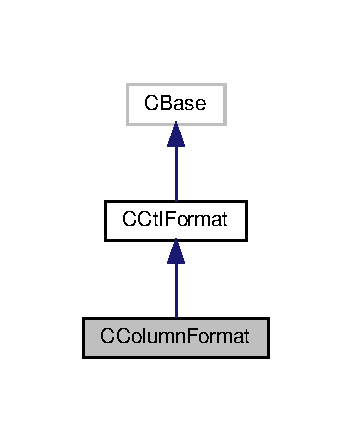
\includegraphics[width=169pt]{classCColumnFormat__inherit__graph}
\end{center}
\end{figure}


Collaboration diagram for C\+Column\+Format\+:
\nopagebreak
\begin{figure}[H]
\begin{center}
\leavevmode
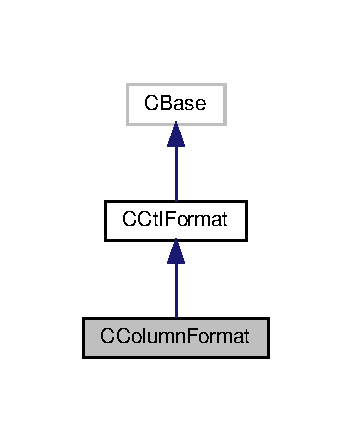
\includegraphics[width=169pt]{classCColumnFormat__coll__graph}
\end{center}
\end{figure}
\subsection*{Public Member Functions}
\begin{DoxyCompactItemize}
\item 
\mbox{\Hypertarget{classCColumnFormat_aae9c5f8938e58fbe682af6ab580b8810}\label{classCColumnFormat_aae9c5f8938e58fbe682af6ab580b8810}} 
\hyperlink{classCColumnFormat}{C\+Column\+Format} $\ast$ {\bfseries Clone} ()
\end{DoxyCompactItemize}
\subsection*{Public Attributes}
\begin{DoxyCompactItemize}
\item 
\mbox{\Hypertarget{classCColumnFormat_a21fb9f9e79dfc4383b4cfe6f04faaaf5}\label{classCColumnFormat_a21fb9f9e79dfc4383b4cfe6f04faaaf5}} 
T\+Int {\bfseries i\+Row\+Height\+In\+Pixels}
\item 
\mbox{\Hypertarget{classCColumnFormat_a03f6122f6dbbfff33df186d3ceac4bdf}\label{classCColumnFormat_a03f6122f6dbbfff33df186d3ceac4bdf}} 
T\+Int {\bfseries i\+Row\+Spacing\+In\+Pixels}
\item 
\mbox{\Hypertarget{classCColumnFormat_aff6fe04dd20c8133662d79ca1dd4d76b}\label{classCColumnFormat_aff6fe04dd20c8133662d79ca1dd4d76b}} 
T\+Int {\bfseries i\+Odd\+Even\+Row\+Dispersion}
\end{DoxyCompactItemize}


The documentation for this class was generated from the following files\+:\begin{DoxyCompactItemize}
\item 
/home/peter/work/github/\+Barba\+G\+U\+I/inc/\+Ctl/Ctl\+Format.\+h\item 
/home/peter/work/github/\+Barba\+G\+U\+I/src/\+Ctl/Ctl\+Format.\+cpp\end{DoxyCompactItemize}

\hypertarget{classCColumnLayout}{}\section{C\+Column\+Layout Class Reference}
\label{classCColumnLayout}\index{C\+Column\+Layout@{C\+Column\+Layout}}


Inheritance diagram for C\+Column\+Layout\+:
\nopagebreak
\begin{figure}[H]
\begin{center}
\leavevmode
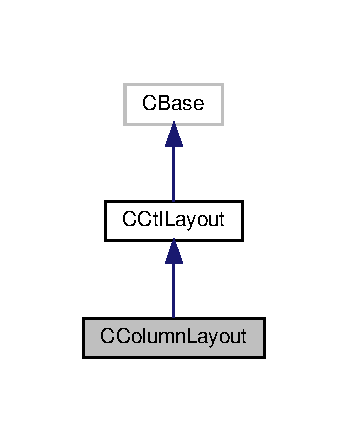
\includegraphics[width=167pt]{classCColumnLayout__inherit__graph}
\end{center}
\end{figure}


Collaboration diagram for C\+Column\+Layout\+:
\nopagebreak
\begin{figure}[H]
\begin{center}
\leavevmode
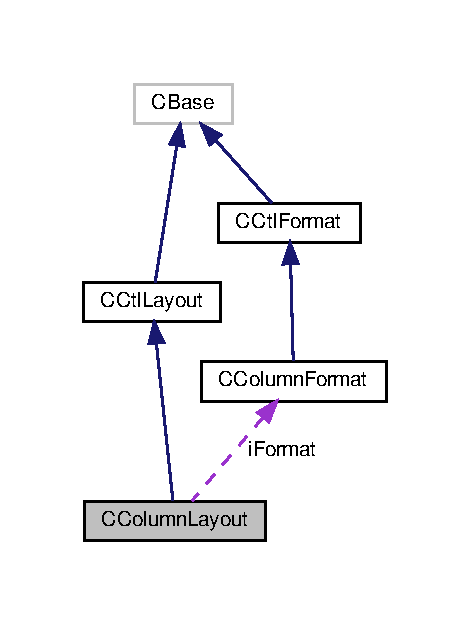
\includegraphics[width=226pt]{classCColumnLayout__coll__graph}
\end{center}
\end{figure}
\subsection*{Public Member Functions}
\begin{DoxyCompactItemize}
\item 
\mbox{\Hypertarget{classCColumnLayout_a1a575b35f5c3a96632fe85dc7d6c0385}\label{classCColumnLayout_a1a575b35f5c3a96632fe85dc7d6c0385}} 
virtual void {\bfseries Get\+Component\+Rect} (const T\+Int a\+Component\+Id, T\+Rect \&a\+Rect) const
\item 
\mbox{\Hypertarget{classCColumnLayout_a285965da00bfee1811a6cc227b4aa83e}\label{classCColumnLayout_a285965da00bfee1811a6cc227b4aa83e}} 
void {\bfseries Set\+Format} (\hyperlink{classCColumnFormat}{C\+Column\+Format} $\ast$a\+Column\+Format)
\end{DoxyCompactItemize}
\subsection*{Protected Attributes}
\begin{DoxyCompactItemize}
\item 
\mbox{\Hypertarget{classCColumnLayout_a132e40e615c3e361b70c6338827574b0}\label{classCColumnLayout_a132e40e615c3e361b70c6338827574b0}} 
\hyperlink{classCColumnFormat}{C\+Column\+Format} $\ast$ {\bfseries i\+Format}
\end{DoxyCompactItemize}


The documentation for this class was generated from the following files\+:\begin{DoxyCompactItemize}
\item 
/home/peter/work/github/\+Barba\+G\+U\+I/inc/\+Ctl/Ctl\+Layout.\+h\item 
/home/peter/work/github/\+Barba\+G\+U\+I/src/\+Ctl/Ctl\+Layout.\+cpp\end{DoxyCompactItemize}

\hypertarget{classCCtlColumn}{}\section{C\+Ctl\+Column Class Reference}
\label{classCCtlColumn}\index{C\+Ctl\+Column@{C\+Ctl\+Column}}


Inheritance diagram for C\+Ctl\+Column\+:
\nopagebreak
\begin{figure}[H]
\begin{center}
\leavevmode
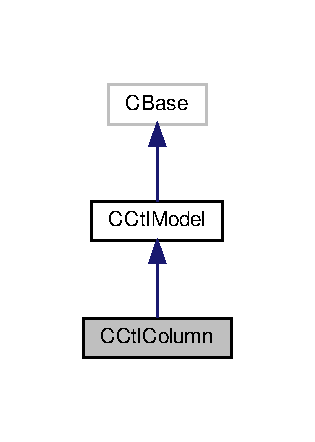
\includegraphics[width=151pt]{classCCtlColumn__inherit__graph}
\end{center}
\end{figure}


Collaboration diagram for C\+Ctl\+Column\+:
\nopagebreak
\begin{figure}[H]
\begin{center}
\leavevmode
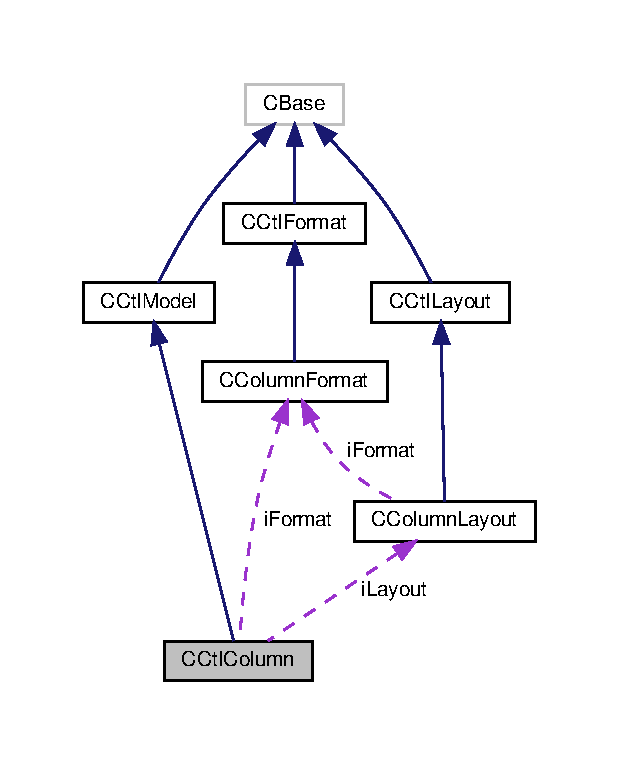
\includegraphics[width=297pt]{classCCtlColumn__coll__graph}
\end{center}
\end{figure}
\subsection*{Public Member Functions}
\begin{DoxyCompactItemize}
\item 
\mbox{\Hypertarget{classCCtlColumn_a53e43b705782cc6e87b254541b54428a}\label{classCCtlColumn_a53e43b705782cc6e87b254541b54428a}} 
virtual void {\bfseries Add} (\hyperlink{classCCtlModel}{C\+Ctl\+Model} $\ast$a\+Ctl\+Model)
\item 
\mbox{\Hypertarget{classCCtlColumn_acd150f2401b0c593e653fe23523d644c}\label{classCCtlColumn_acd150f2401b0c593e653fe23523d644c}} 
virtual void {\bfseries Remove} (T\+Int an\+Index)
\item 
\mbox{\Hypertarget{classCCtlColumn_a9eeb51471aa301aca4659b44f1e06b86}\label{classCCtlColumn_a9eeb51471aa301aca4659b44f1e06b86}} 
virtual T\+Int {\bfseries Insert} (\hyperlink{classCCtlModel}{C\+Ctl\+Model} $\ast$a\+Ctl\+Model, T\+Int a\+Pos)
\item 
\mbox{\Hypertarget{classCCtlColumn_a14e0f5d0a85cee79330493369e2e119b}\label{classCCtlColumn_a14e0f5d0a85cee79330493369e2e119b}} 
virtual void {\bfseries Reset} ()
\item 
\mbox{\Hypertarget{classCCtlColumn_a494608a7b5783174f846b6f4f6fd02e6}\label{classCCtlColumn_a494608a7b5783174f846b6f4f6fd02e6}} 
virtual T\+Int {\bfseries Count} ()
\item 
\mbox{\Hypertarget{classCCtlColumn_a17465d6905c7edd344501482328266ed}\label{classCCtlColumn_a17465d6905c7edd344501482328266ed}} 
virtual void {\bfseries Draw} (C\+Window\+Gc \&gc, const T\+Rect $\ast$a\+Rect) const
\item 
\mbox{\Hypertarget{classCCtlColumn_a777f49862d0987da6cc24b39764456a1}\label{classCCtlColumn_a777f49862d0987da6cc24b39764456a1}} 
virtual void {\bfseries Make\+Visible} (T\+Bool a\+Visible)
\item 
\mbox{\Hypertarget{classCCtlColumn_a2a6a9b186bc0688b15e32ed72bd6b8c2}\label{classCCtlColumn_a2a6a9b186bc0688b15e32ed72bd6b8c2}} 
virtual \hyperlink{classCCtlModel}{C\+Ctl\+Model} $\ast$ {\bfseries At} (T\+Int a\+Index)
\item 
\mbox{\Hypertarget{classCCtlColumn_a9d8c4c9a055229c2c5c7c00fa7c50cf2}\label{classCCtlColumn_a9d8c4c9a055229c2c5c7c00fa7c50cf2}} 
virtual \hyperlink{classCCtlModel}{C\+Ctl\+Model} $\ast$ {\bfseries Clone} ()
\item 
\mbox{\Hypertarget{classCCtlColumn_ac1f1643f1a63b3459dce276c8b0bdc61}\label{classCCtlColumn_ac1f1643f1a63b3459dce276c8b0bdc61}} 
virtual \hyperlink{classCCtlModel}{C\+Ctl\+Model} $\ast$ {\bfseries Clone3D} ()
\item 
\mbox{\Hypertarget{classCCtlColumn_a2e495e9cc31e46a69b2b50385dce3a41}\label{classCCtlColumn_a2e495e9cc31e46a69b2b50385dce3a41}} 
virtual T\+Rect $\ast$ {\bfseries Rect} () const
\item 
\mbox{\Hypertarget{classCCtlColumn_a9dbfc8e92af000b797616c19ca28215d}\label{classCCtlColumn_a9dbfc8e92af000b797616c19ca28215d}} 
void {\bfseries Set\+Rect} (const T\+Rect \&a\+Rect)
\item 
\mbox{\Hypertarget{classCCtlColumn_a7c95cd8f2de20cd9b2ee0790fe0697ac}\label{classCCtlColumn_a7c95cd8f2de20cd9b2ee0790fe0697ac}} 
void {\bfseries Set\+View\+Rect} (const T\+Rect \&a\+Rect)
\item 
\mbox{\Hypertarget{classCCtlColumn_a73b42fcf69b77e1846f2758c1ab628f5}\label{classCCtlColumn_a73b42fcf69b77e1846f2758c1ab628f5}} 
void {\bfseries Set\+Layout} (\hyperlink{classCColumnLayout}{C\+Column\+Layout} $\ast$a\+Layout)
\item 
\mbox{\Hypertarget{classCCtlColumn_a193abd36446de5d62c98371ca32a3ef8}\label{classCCtlColumn_a193abd36446de5d62c98371ca32a3ef8}} 
\hyperlink{classCColumnFormat}{C\+Column\+Format} $\ast$ {\bfseries Format} ()
\item 
\mbox{\Hypertarget{classCCtlColumn_a30b63b99ec2facdc20b7f5fc1dfce206}\label{classCCtlColumn_a30b63b99ec2facdc20b7f5fc1dfce206}} 
void {\bfseries Set\+Format} (\hyperlink{classCColumnFormat}{C\+Column\+Format} $\ast$a\+Format)
\item 
\mbox{\Hypertarget{classCCtlColumn_a2049d52d628f7bf397590598f0b2487b}\label{classCCtlColumn_a2049d52d628f7bf397590598f0b2487b}} 
T\+Int {\bfseries Selection} ()
\item 
\mbox{\Hypertarget{classCCtlColumn_ad61bf3caf2b89472e73f38ddcb31b492}\label{classCCtlColumn_ad61bf3caf2b89472e73f38ddcb31b492}} 
T\+Int {\bfseries Get\+Selection} (const T\+Point \&a\+Point)
\item 
\mbox{\Hypertarget{classCCtlColumn_a29de877103fc2ad3c3beb260339f506b}\label{classCCtlColumn_a29de877103fc2ad3c3beb260339f506b}} 
void {\bfseries Set\+Selection} (T\+Int a\+Index)
\item 
\mbox{\Hypertarget{classCCtlColumn_a8d489581a0a3611eabaa8b91ea3490d4}\label{classCCtlColumn_a8d489581a0a3611eabaa8b91ea3490d4}} 
virtual void {\bfseries Do\+Select} (\hyperlink{classCCtlModel}{C\+Ctl\+Model} $\ast$a\+Source, C\+Window\+Gc \&gc, const T\+Rect $\ast$a\+Rect) const
\item 
\mbox{\Hypertarget{classCCtlColumn_a9b212e5aac3197c793e9603991e0718d}\label{classCCtlColumn_a9b212e5aac3197c793e9603991e0718d}} 
T\+Int {\bfseries Components\+Count} ()
\item 
\mbox{\Hypertarget{classCCtlColumn_aab6e1ffad97860cd859a739f90ec2cec}\label{classCCtlColumn_aab6e1ffad97860cd859a739f90ec2cec}} 
virtual T\+Int {\bfseries Visible\+Top\+Line} ()
\item 
\mbox{\Hypertarget{classCCtlColumn_affcbebd8b7280a8862d7eecfcd9ff4c1}\label{classCCtlColumn_affcbebd8b7280a8862d7eecfcd9ff4c1}} 
virtual T\+Int {\bfseries Visible\+Bottom\+Line} ()
\end{DoxyCompactItemize}
\subsection*{Static Public Member Functions}
\begin{DoxyCompactItemize}
\item 
\mbox{\Hypertarget{classCCtlColumn_a77ec2692f144f3a75e61d91ba6ddd98b}\label{classCCtlColumn_a77ec2692f144f3a75e61d91ba6ddd98b}} 
static \hyperlink{classCCtlColumn}{C\+Ctl\+Column} $\ast$ {\bfseries NewL} ()
\item 
\mbox{\Hypertarget{classCCtlColumn_a4e7afa16a28869b5c3fbbf232f360bad}\label{classCCtlColumn_a4e7afa16a28869b5c3fbbf232f360bad}} 
static \hyperlink{classCCtlColumn}{C\+Ctl\+Column} $\ast$ {\bfseries New\+LC} ()
\end{DoxyCompactItemize}
\subsection*{Protected Member Functions}
\begin{DoxyCompactItemize}
\item 
\mbox{\Hypertarget{classCCtlColumn_a20b96fb8d56714c1555b98d749e6fea9}\label{classCCtlColumn_a20b96fb8d56714c1555b98d749e6fea9}} 
void {\bfseries ConstructL} ()
\end{DoxyCompactItemize}
\subsection*{Protected Attributes}
\begin{DoxyCompactItemize}
\item 
\mbox{\Hypertarget{classCCtlColumn_a1ac8951c3a1c3e7c5a7ed602f999303d}\label{classCCtlColumn_a1ac8951c3a1c3e7c5a7ed602f999303d}} 
R\+Pointer\+Array$<$ \hyperlink{classCCtlModel}{C\+Ctl\+Model} $>$ $\ast$ {\bfseries i\+Components}
\item 
\mbox{\Hypertarget{classCCtlColumn_ab81f9bd0162887c5b5623889b6721986}\label{classCCtlColumn_ab81f9bd0162887c5b5623889b6721986}} 
\hyperlink{classCColumnFormat}{C\+Column\+Format} $\ast$ {\bfseries i\+Format}
\item 
\mbox{\Hypertarget{classCCtlColumn_af37930eaaac60c35b08b0b49a38a4808}\label{classCCtlColumn_af37930eaaac60c35b08b0b49a38a4808}} 
\hyperlink{classCColumnLayout}{C\+Column\+Layout} $\ast$ {\bfseries i\+Layout}
\item 
\mbox{\Hypertarget{classCCtlColumn_ab5642a466e4cc4ec869e5729bfadf406}\label{classCCtlColumn_ab5642a466e4cc4ec869e5729bfadf406}} 
T\+Bool {\bfseries i\+Visible}
\item 
\mbox{\Hypertarget{classCCtlColumn_a0f5586dda0bc3cc1b688c72c8cd5ed34}\label{classCCtlColumn_a0f5586dda0bc3cc1b688c72c8cd5ed34}} 
T\+Int {\bfseries i\+Selected\+Index}
\end{DoxyCompactItemize}


The documentation for this class was generated from the following files\+:\begin{DoxyCompactItemize}
\item 
/home/peter/work/github/\+Barba\+G\+U\+I/inc/\+Ctl/Ctl\+Column.\+h\item 
/home/peter/work/github/\+Barba\+G\+U\+I/src/\+Ctl/Ctl\+Column.\+cpp\end{DoxyCompactItemize}

\hypertarget{classCCtlFormat}{}\section{C\+Ctl\+Format Class Reference}
\label{classCCtlFormat}\index{C\+Ctl\+Format@{C\+Ctl\+Format}}


Inheritance diagram for C\+Ctl\+Format\+:
\nopagebreak
\begin{figure}[H]
\begin{center}
\leavevmode
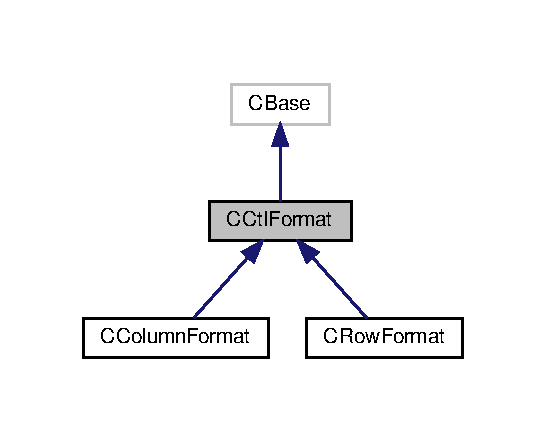
\includegraphics[width=262pt]{classCCtlFormat__inherit__graph}
\end{center}
\end{figure}


Collaboration diagram for C\+Ctl\+Format\+:
\nopagebreak
\begin{figure}[H]
\begin{center}
\leavevmode
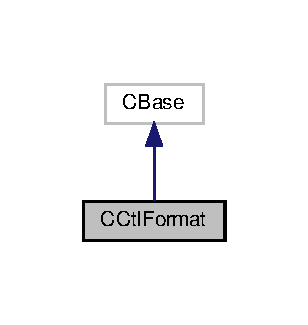
\includegraphics[width=148pt]{classCCtlFormat__coll__graph}
\end{center}
\end{figure}
\subsection*{Public Attributes}
\begin{DoxyCompactItemize}
\item 
\mbox{\Hypertarget{classCCtlFormat_aadcdbf14d17e5e446173b407307fab3b}\label{classCCtlFormat_aadcdbf14d17e5e446173b407307fab3b}} 
T\+Rect {\bfseries i\+Rect}
\item 
\mbox{\Hypertarget{classCCtlFormat_aca9e1ea2253d12e69f7db0ae7e79b94f}\label{classCCtlFormat_aca9e1ea2253d12e69f7db0ae7e79b94f}} 
T\+Rect {\bfseries i\+View\+Rect}
\item 
\mbox{\Hypertarget{classCCtlFormat_a1c657d2edf7d6196d4ddbf4820e388ea}\label{classCCtlFormat_a1c657d2edf7d6196d4ddbf4820e388ea}} 
T\+Int {\bfseries i\+Left\+Margin\+In\+Pixels}
\item 
\mbox{\Hypertarget{classCCtlFormat_a9005ff7384eef41913705eace5b5b791}\label{classCCtlFormat_a9005ff7384eef41913705eace5b5b791}} 
T\+Int {\bfseries i\+Right\+Margin\+In\+Pixels}
\item 
\mbox{\Hypertarget{classCCtlFormat_aab1d7db3ab83a8e38218ca820455963d}\label{classCCtlFormat_aab1d7db3ab83a8e38218ca820455963d}} 
T\+Int {\bfseries i\+Top\+Margin\+In\+Pixels}
\item 
\mbox{\Hypertarget{classCCtlFormat_aba2f8ae6c857c1b9c6ffb3b1da95810b}\label{classCCtlFormat_aba2f8ae6c857c1b9c6ffb3b1da95810b}} 
T\+Int {\bfseries i\+Bottom\+Margin\+In\+Pixels}
\end{DoxyCompactItemize}


The documentation for this class was generated from the following file\+:\begin{DoxyCompactItemize}
\item 
/home/peter/work/github/\+Barba\+G\+U\+I/inc/\+Ctl/Ctl\+Format.\+h\end{DoxyCompactItemize}

\hypertarget{classCCtlGraphic}{}\section{C\+Ctl\+Graphic Class Reference}
\label{classCCtlGraphic}\index{C\+Ctl\+Graphic@{C\+Ctl\+Graphic}}


Inheritance diagram for C\+Ctl\+Graphic\+:
\nopagebreak
\begin{figure}[H]
\begin{center}
\leavevmode
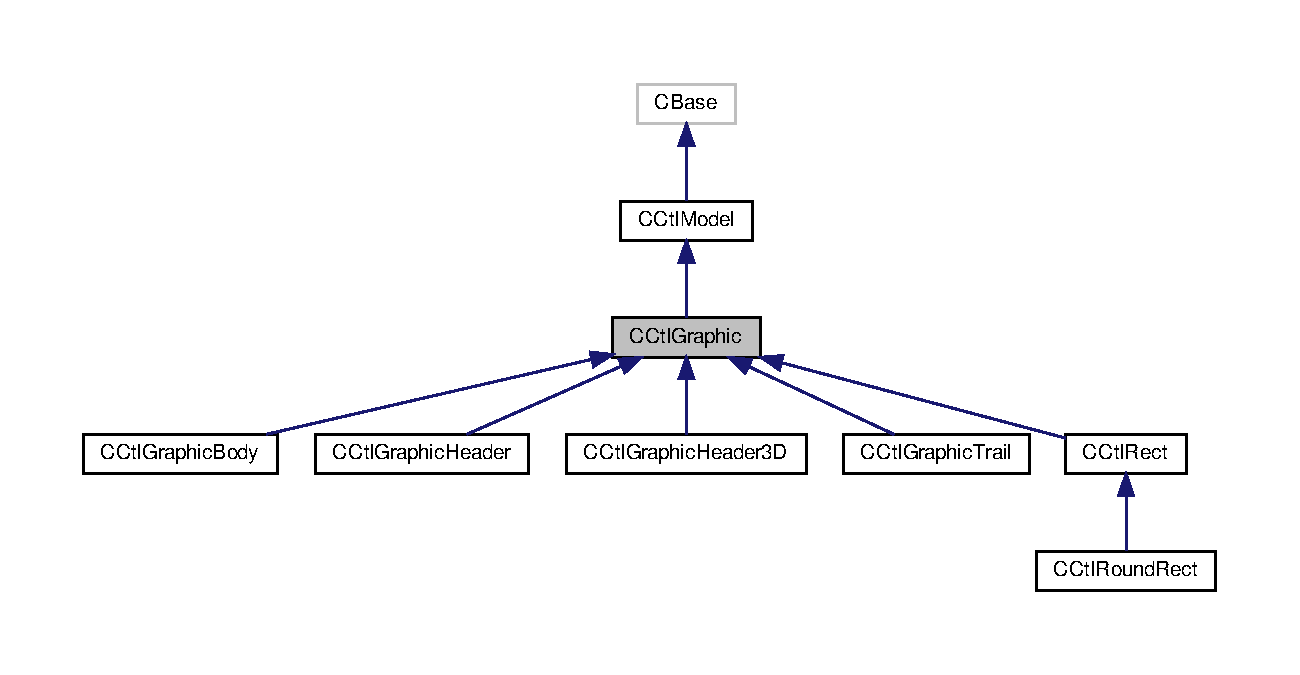
\includegraphics[width=350pt]{classCCtlGraphic__inherit__graph}
\end{center}
\end{figure}


Collaboration diagram for C\+Ctl\+Graphic\+:
\nopagebreak
\begin{figure}[H]
\begin{center}
\leavevmode
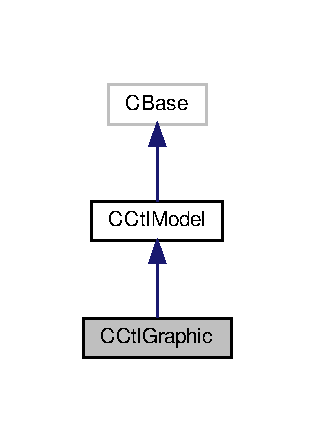
\includegraphics[width=151pt]{classCCtlGraphic__coll__graph}
\end{center}
\end{figure}
\subsection*{Public Types}
\begin{DoxyCompactItemize}
\item 
\mbox{\Hypertarget{classCCtlGraphic_aef9f8dddf738a51d4493f06236210146}\label{classCCtlGraphic_aef9f8dddf738a51d4493f06236210146}} 
enum {\bfseries T\+Graphic\+Type} \{ {\bfseries E\+Header}, 
{\bfseries E\+Body}, 
{\bfseries E\+Trail}, 
{\bfseries E\+Round\+Rect}
 \}
\end{DoxyCompactItemize}
\subsection*{Additional Inherited Members}


The documentation for this class was generated from the following file\+:\begin{DoxyCompactItemize}
\item 
/home/peter/work/github/\+Barba\+G\+U\+I/inc/\+Ctl/Ctl\+Graphic.\+h\end{DoxyCompactItemize}

\hypertarget{classCCtlGraphicBody}{}\section{C\+Ctl\+Graphic\+Body Class Reference}
\label{classCCtlGraphicBody}\index{C\+Ctl\+Graphic\+Body@{C\+Ctl\+Graphic\+Body}}


Inheritance diagram for C\+Ctl\+Graphic\+Body\+:
\nopagebreak
\begin{figure}[H]
\begin{center}
\leavevmode
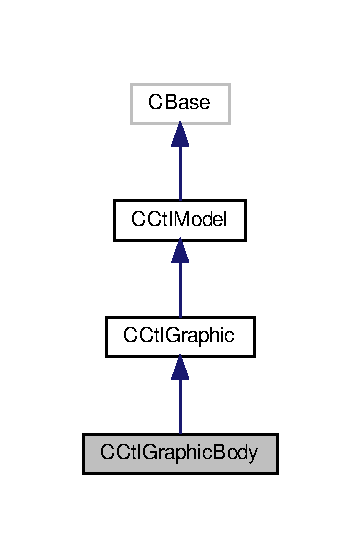
\includegraphics[width=173pt]{classCCtlGraphicBody__inherit__graph}
\end{center}
\end{figure}


Collaboration diagram for C\+Ctl\+Graphic\+Body\+:
\nopagebreak
\begin{figure}[H]
\begin{center}
\leavevmode
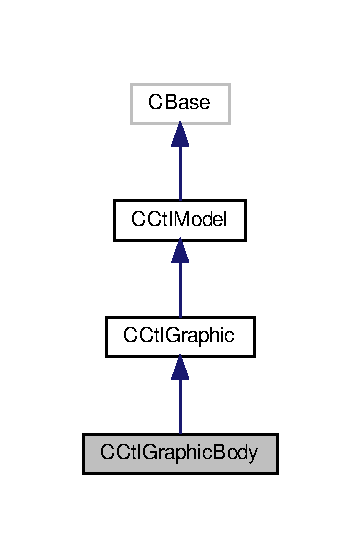
\includegraphics[width=173pt]{classCCtlGraphicBody__coll__graph}
\end{center}
\end{figure}
\subsection*{Public Member Functions}
\begin{DoxyCompactItemize}
\item 
\mbox{\Hypertarget{classCCtlGraphicBody_ab72452232681db8b83338e494c514e52}\label{classCCtlGraphicBody_ab72452232681db8b83338e494c514e52}} 
\hyperlink{classCCtlGraphicBody_ab72452232681db8b83338e494c514e52}{C\+Ctl\+Graphic\+Body} (T\+Rgb a\+Brush\+Color, T\+Rgb a\+Line\+Color)
\begin{DoxyCompactList}\small\item\em \hyperlink{classCCtlGraphicBody}{C\+Ctl\+Graphic\+Body}. \end{DoxyCompactList}\item 
\mbox{\Hypertarget{classCCtlGraphicBody_aa9941adefbe2d6b52e3ea908fb900571}\label{classCCtlGraphicBody_aa9941adefbe2d6b52e3ea908fb900571}} 
virtual \hyperlink{classCCtlModel}{C\+Ctl\+Model} $\ast$ {\bfseries Clone} ()
\item 
\mbox{\Hypertarget{classCCtlGraphicBody_a8a9f6c7dc81473e81efb462aae43c3fc}\label{classCCtlGraphicBody_a8a9f6c7dc81473e81efb462aae43c3fc}} 
virtual \hyperlink{classCCtlModel}{C\+Ctl\+Model} $\ast$ {\bfseries Clone3D} ()
\item 
\mbox{\Hypertarget{classCCtlGraphicBody_a54172fb69837af17afcf09fa0ca050c9}\label{classCCtlGraphicBody_a54172fb69837af17afcf09fa0ca050c9}} 
virtual void {\bfseries Draw} (C\+Window\+Gc \&gc, const T\+Rect $\ast$a\+Rect) const
\end{DoxyCompactItemize}
\subsection*{Additional Inherited Members}


The documentation for this class was generated from the following files\+:\begin{DoxyCompactItemize}
\item 
/home/peter/work/github/\+Barba\+G\+U\+I/inc/\+Ctl/Ctl\+Graphic.\+h\item 
/home/peter/work/github/\+Barba\+G\+U\+I/src/\+Ctl/Ctl\+Graphic.\+cpp\end{DoxyCompactItemize}

\hypertarget{classCCtlGraphicHeader}{}\section{C\+Ctl\+Graphic\+Header Class Reference}
\label{classCCtlGraphicHeader}\index{C\+Ctl\+Graphic\+Header@{C\+Ctl\+Graphic\+Header}}


Inheritance diagram for C\+Ctl\+Graphic\+Header\+:
\nopagebreak
\begin{figure}[H]
\begin{center}
\leavevmode
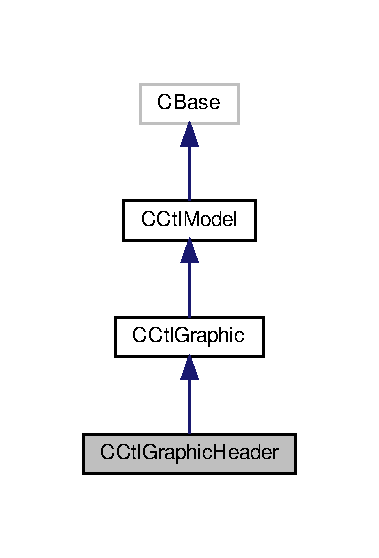
\includegraphics[width=182pt]{classCCtlGraphicHeader__inherit__graph}
\end{center}
\end{figure}


Collaboration diagram for C\+Ctl\+Graphic\+Header\+:
\nopagebreak
\begin{figure}[H]
\begin{center}
\leavevmode
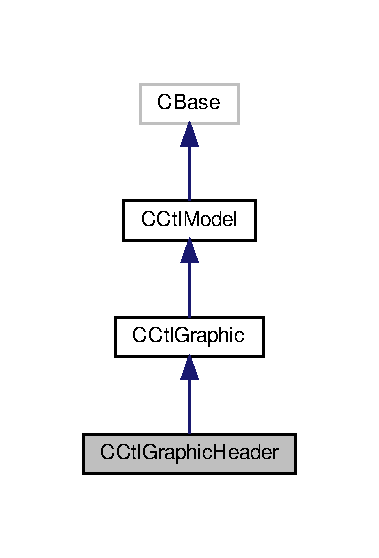
\includegraphics[width=182pt]{classCCtlGraphicHeader__coll__graph}
\end{center}
\end{figure}
\subsection*{Public Member Functions}
\begin{DoxyCompactItemize}
\item 
\mbox{\Hypertarget{classCCtlGraphicHeader_abffa970ad7c3ee275afebd7e595c7b8c}\label{classCCtlGraphicHeader_abffa970ad7c3ee275afebd7e595c7b8c}} 
virtual \hyperlink{classCCtlModel}{C\+Ctl\+Model} $\ast$ {\bfseries Clone} ()
\item 
\mbox{\Hypertarget{classCCtlGraphicHeader_a05e1739009760c0b7ac25dbc24e2cb38}\label{classCCtlGraphicHeader_a05e1739009760c0b7ac25dbc24e2cb38}} 
virtual \hyperlink{classCCtlModel}{C\+Ctl\+Model} $\ast$ {\bfseries Clone3D} ()
\item 
\mbox{\Hypertarget{classCCtlGraphicHeader_a2e00efa368b078c10db3a85b8aeacc88}\label{classCCtlGraphicHeader_a2e00efa368b078c10db3a85b8aeacc88}} 
virtual void {\bfseries Draw} (C\+Window\+Gc \&gc, const T\+Rect $\ast$a\+Rect) const
\item 
\mbox{\Hypertarget{classCCtlGraphicHeader_a638b8b91ae973c47f75291cd82b3129b}\label{classCCtlGraphicHeader_a638b8b91ae973c47f75291cd82b3129b}} 
\hyperlink{classCCtlGraphicHeader_a638b8b91ae973c47f75291cd82b3129b}{C\+Ctl\+Graphic\+Header} (T\+Rgb a\+Brush\+Color, T\+Rgb a\+Line\+Color)
\begin{DoxyCompactList}\small\item\em \hyperlink{classCCtlGraphicHeader}{C\+Ctl\+Graphic\+Header}. \end{DoxyCompactList}\end{DoxyCompactItemize}
\subsection*{Additional Inherited Members}


The documentation for this class was generated from the following files\+:\begin{DoxyCompactItemize}
\item 
/home/peter/work/github/\+Barba\+G\+U\+I/inc/\+Ctl/Ctl\+Graphic.\+h\item 
/home/peter/work/github/\+Barba\+G\+U\+I/src/\+Ctl/Ctl\+Graphic.\+cpp\end{DoxyCompactItemize}

\hypertarget{classCCtlGraphicHeader3D}{}\section{C\+Ctl\+Graphic\+Header3D Class Reference}
\label{classCCtlGraphicHeader3D}\index{C\+Ctl\+Graphic\+Header3D@{C\+Ctl\+Graphic\+Header3D}}


Inheritance diagram for C\+Ctl\+Graphic\+Header3D\+:
\nopagebreak
\begin{figure}[H]
\begin{center}
\leavevmode
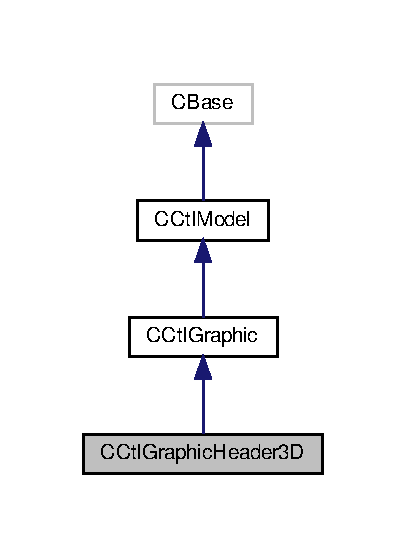
\includegraphics[width=195pt]{classCCtlGraphicHeader3D__inherit__graph}
\end{center}
\end{figure}


Collaboration diagram for C\+Ctl\+Graphic\+Header3D\+:
\nopagebreak
\begin{figure}[H]
\begin{center}
\leavevmode
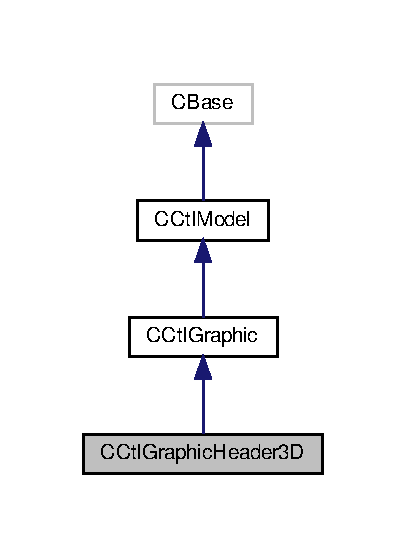
\includegraphics[width=195pt]{classCCtlGraphicHeader3D__coll__graph}
\end{center}
\end{figure}
\subsection*{Public Member Functions}
\begin{DoxyCompactItemize}
\item 
\mbox{\Hypertarget{classCCtlGraphicHeader3D_ab264d0e210428a2496ff927509e334c2}\label{classCCtlGraphicHeader3D_ab264d0e210428a2496ff927509e334c2}} 
virtual \hyperlink{classCCtlModel}{C\+Ctl\+Model} $\ast$ {\bfseries Clone} ()
\item 
\mbox{\Hypertarget{classCCtlGraphicHeader3D_acfc7df2bcec257ac7313d52c782eb23a}\label{classCCtlGraphicHeader3D_acfc7df2bcec257ac7313d52c782eb23a}} 
virtual \hyperlink{classCCtlModel}{C\+Ctl\+Model} $\ast$ {\bfseries Clone3D} ()
\item 
\mbox{\Hypertarget{classCCtlGraphicHeader3D_a3253d46cdf047f1b0f477bc14a5971e2}\label{classCCtlGraphicHeader3D_a3253d46cdf047f1b0f477bc14a5971e2}} 
virtual void {\bfseries Draw} (C\+Window\+Gc \&gc, const T\+Rect $\ast$a\+Rect) const
\item 
\mbox{\Hypertarget{classCCtlGraphicHeader3D_a21f6dd3abfa1c0db522bc17659d62f89}\label{classCCtlGraphicHeader3D_a21f6dd3abfa1c0db522bc17659d62f89}} 
\hyperlink{classCCtlGraphicHeader3D_a21f6dd3abfa1c0db522bc17659d62f89}{C\+Ctl\+Graphic\+Header3D} (T\+Rgb a\+Line\+Color)
\begin{DoxyCompactList}\small\item\em \hyperlink{classCCtlGraphicHeader3D}{C\+Ctl\+Graphic\+Header3D}. \end{DoxyCompactList}\end{DoxyCompactItemize}
\subsection*{Additional Inherited Members}


The documentation for this class was generated from the following files\+:\begin{DoxyCompactItemize}
\item 
/home/peter/work/github/\+Barba\+G\+U\+I/inc/\+Ctl/Ctl\+Graphic.\+h\item 
/home/peter/work/github/\+Barba\+G\+U\+I/src/\+Ctl/Ctl\+Graphic.\+cpp\end{DoxyCompactItemize}

\hypertarget{classCCtlGraphicTrail}{}\section{C\+Ctl\+Graphic\+Trail Class Reference}
\label{classCCtlGraphicTrail}\index{C\+Ctl\+Graphic\+Trail@{C\+Ctl\+Graphic\+Trail}}


Inheritance diagram for C\+Ctl\+Graphic\+Trail\+:
\nopagebreak
\begin{figure}[H]
\begin{center}
\leavevmode
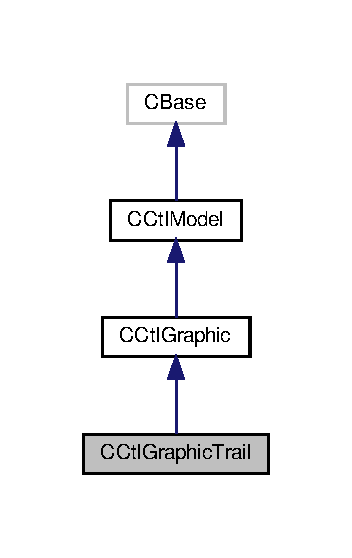
\includegraphics[width=169pt]{classCCtlGraphicTrail__inherit__graph}
\end{center}
\end{figure}


Collaboration diagram for C\+Ctl\+Graphic\+Trail\+:
\nopagebreak
\begin{figure}[H]
\begin{center}
\leavevmode
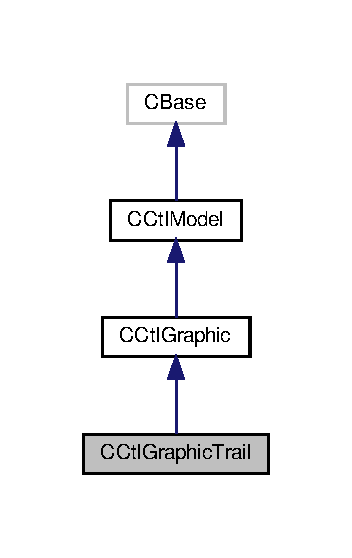
\includegraphics[width=169pt]{classCCtlGraphicTrail__coll__graph}
\end{center}
\end{figure}
\subsection*{Public Member Functions}
\begin{DoxyCompactItemize}
\item 
\mbox{\Hypertarget{classCCtlGraphicTrail_a7f8ed409fd4c8027438fbd0ca5cba297}\label{classCCtlGraphicTrail_a7f8ed409fd4c8027438fbd0ca5cba297}} 
virtual \hyperlink{classCCtlModel}{C\+Ctl\+Model} $\ast$ {\bfseries Clone} ()
\item 
\mbox{\Hypertarget{classCCtlGraphicTrail_a4aba0b897053b0ffe46172d7370cacad}\label{classCCtlGraphicTrail_a4aba0b897053b0ffe46172d7370cacad}} 
virtual \hyperlink{classCCtlModel}{C\+Ctl\+Model} $\ast$ {\bfseries Clone3D} ()
\item 
\mbox{\Hypertarget{classCCtlGraphicTrail_a742d5371a7ef9f1f88b03e77a8b5dc3a}\label{classCCtlGraphicTrail_a742d5371a7ef9f1f88b03e77a8b5dc3a}} 
virtual void {\bfseries Draw} (C\+Window\+Gc \&gc, const T\+Rect $\ast$a\+Rect) const
\item 
\mbox{\Hypertarget{classCCtlGraphicTrail_ad28ad0da08194efb9b310bcf3e5d94ac}\label{classCCtlGraphicTrail_ad28ad0da08194efb9b310bcf3e5d94ac}} 
\hyperlink{classCCtlGraphicTrail_ad28ad0da08194efb9b310bcf3e5d94ac}{C\+Ctl\+Graphic\+Trail} (T\+Rgb a\+Brush\+Color, T\+Rgb a\+Line\+Color)
\begin{DoxyCompactList}\small\item\em \hyperlink{classCCtlGraphicTrail}{C\+Ctl\+Graphic\+Trail}. \end{DoxyCompactList}\end{DoxyCompactItemize}
\subsection*{Additional Inherited Members}


The documentation for this class was generated from the following files\+:\begin{DoxyCompactItemize}
\item 
/home/peter/work/github/\+Barba\+G\+U\+I/inc/\+Ctl/Ctl\+Graphic.\+h\item 
/home/peter/work/github/\+Barba\+G\+U\+I/src/\+Ctl/Ctl\+Graphic.\+cpp\end{DoxyCompactItemize}

\hypertarget{classCCtlLayout}{}\section{C\+Ctl\+Layout Class Reference}
\label{classCCtlLayout}\index{C\+Ctl\+Layout@{C\+Ctl\+Layout}}


Inheritance diagram for C\+Ctl\+Layout\+:
\nopagebreak
\begin{figure}[H]
\begin{center}
\leavevmode
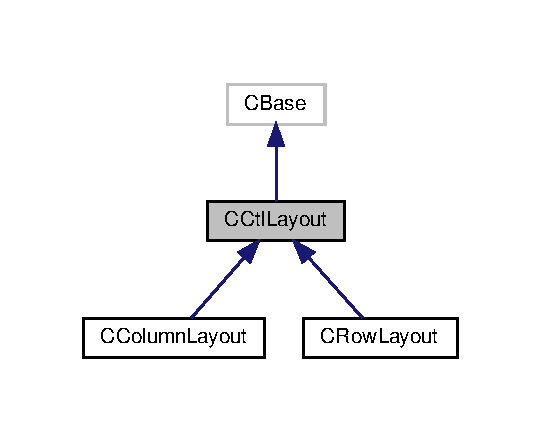
\includegraphics[width=260pt]{classCCtlLayout__inherit__graph}
\end{center}
\end{figure}


Collaboration diagram for C\+Ctl\+Layout\+:
\nopagebreak
\begin{figure}[H]
\begin{center}
\leavevmode
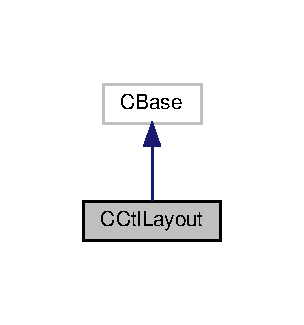
\includegraphics[width=146pt]{classCCtlLayout__coll__graph}
\end{center}
\end{figure}
\subsection*{Public Member Functions}
\begin{DoxyCompactItemize}
\item 
\mbox{\Hypertarget{classCCtlLayout_ab1bc3fda6d4d757a2a2216025376538d}\label{classCCtlLayout_ab1bc3fda6d4d757a2a2216025376538d}} 
virtual void {\bfseries Do\+Layout} (const T\+Rect \&) const
\item 
\mbox{\Hypertarget{classCCtlLayout_ae1000493c85b64d4bb8fada61dcea588}\label{classCCtlLayout_ae1000493c85b64d4bb8fada61dcea588}} 
virtual void {\bfseries Get\+Component\+Rect} (const T\+Int a\+Component\+Id, T\+Rect \&a\+Rect) const
\end{DoxyCompactItemize}


The documentation for this class was generated from the following file\+:\begin{DoxyCompactItemize}
\item 
/home/peter/work/github/\+Barba\+G\+U\+I/inc/\+Ctl/Ctl\+Layout.\+h\end{DoxyCompactItemize}

\hypertarget{classCCtlListBox}{}\section{C\+Ctl\+List\+Box Class Reference}
\label{classCCtlListBox}\index{C\+Ctl\+List\+Box@{C\+Ctl\+List\+Box}}


Collaboration diagram for C\+Ctl\+List\+Box\+:
\nopagebreak
\begin{figure}[H]
\begin{center}
\leavevmode
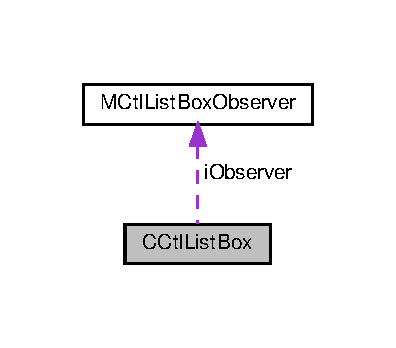
\includegraphics[width=190pt]{classCCtlListBox__coll__graph}
\end{center}
\end{figure}
\subsection*{Public Member Functions}
\begin{DoxyCompactItemize}
\item 
\mbox{\Hypertarget{classCCtlListBox_a3d64c3d1fd6826c3a8a55f617cda6904}\label{classCCtlListBox_a3d64c3d1fd6826c3a8a55f617cda6904}} 
\hyperlink{classMCtlListBoxObserver}{M\+Ctl\+List\+Box\+Observer} $\ast$ {\bfseries Observer} ()
\item 
\mbox{\Hypertarget{classCCtlListBox_a86982ba163f5a2514b44a7709ffa3dc3}\label{classCCtlListBox_a86982ba163f5a2514b44a7709ffa3dc3}} 
void {\bfseries Set\+Observer} (\hyperlink{classMCtlListBoxObserver}{M\+Ctl\+List\+Box\+Observer} $\ast$a\+Observer)
\item 
\mbox{\Hypertarget{classCCtlListBox_aec654fe85618626641637761d3d7d862}\label{classCCtlListBox_aec654fe85618626641637761d3d7d862}} 
T\+Int {\bfseries Append\+Icon} (C\+Gul\+Icon $\ast$a\+Gul\+Icon)
\end{DoxyCompactItemize}
\subsection*{Protected Attributes}
\begin{DoxyCompactItemize}
\item 
\mbox{\Hypertarget{classCCtlListBox_ac5ee8c1b8996be8d5382b2d187925811}\label{classCCtlListBox_ac5ee8c1b8996be8d5382b2d187925811}} 
\hyperlink{classMCtlListBoxObserver}{M\+Ctl\+List\+Box\+Observer} $\ast$ {\bfseries i\+Observer}
\item 
\mbox{\Hypertarget{classCCtlListBox_a4a936e5121611964ac32c7e79723bc57}\label{classCCtlListBox_a4a936e5121611964ac32c7e79723bc57}} 
R\+Pointer\+Array$<$ C\+Gul\+Icon $>$ {\bfseries i\+Icon\+Array}
\end{DoxyCompactItemize}


The documentation for this class was generated from the following files\+:\begin{DoxyCompactItemize}
\item 
/home/peter/work/github/\+Barba\+G\+U\+I/inc/\+Ctl/Ctl\+List\+Box.\+h\item 
/home/peter/work/github/\+Barba\+G\+U\+I/src/\+Ctl/Ctl\+List\+Box.\+cpp\end{DoxyCompactItemize}

\hypertarget{classCCtlModel}{}\section{C\+Ctl\+Model Class Reference}
\label{classCCtlModel}\index{C\+Ctl\+Model@{C\+Ctl\+Model}}


Inheritance diagram for C\+Ctl\+Model\+:
\nopagebreak
\begin{figure}[H]
\begin{center}
\leavevmode
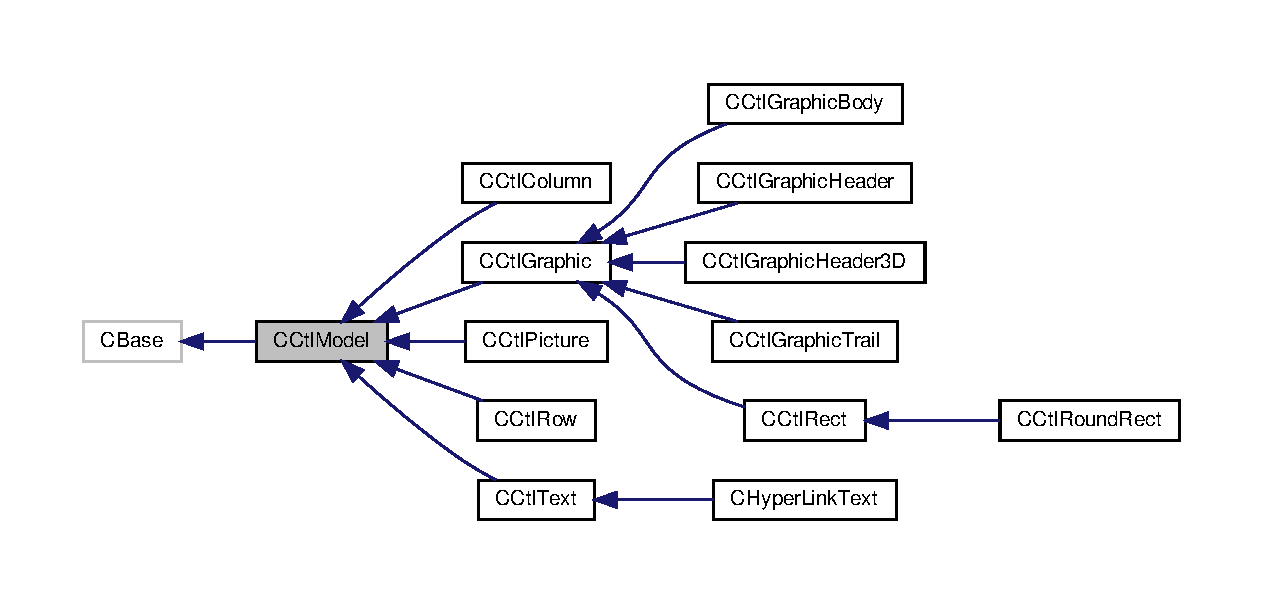
\includegraphics[width=350pt]{classCCtlModel__inherit__graph}
\end{center}
\end{figure}


Collaboration diagram for C\+Ctl\+Model\+:
\nopagebreak
\begin{figure}[H]
\begin{center}
\leavevmode
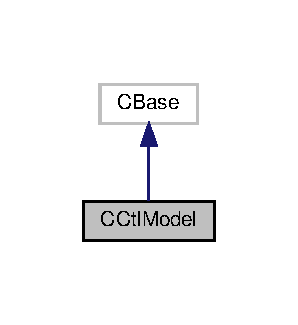
\includegraphics[width=143pt]{classCCtlModel__coll__graph}
\end{center}
\end{figure}
\subsection*{Public Member Functions}
\begin{DoxyCompactItemize}
\item 
\mbox{\Hypertarget{classCCtlModel_a965f60b58d4acf4255bac06ac25d59d3}\label{classCCtlModel_a965f60b58d4acf4255bac06ac25d59d3}} 
virtual void {\bfseries Add} (\hyperlink{classCCtlModel}{C\+Ctl\+Model} $\ast$)
\item 
\mbox{\Hypertarget{classCCtlModel_aa441740adf43f79ec136d05c55267cd2}\label{classCCtlModel_aa441740adf43f79ec136d05c55267cd2}} 
virtual void {\bfseries Remove} (T\+Int)
\item 
\mbox{\Hypertarget{classCCtlModel_affe0c82f78c498d112a815c20b54b79b}\label{classCCtlModel_affe0c82f78c498d112a815c20b54b79b}} 
virtual T\+Int {\bfseries Insert} (\hyperlink{classCCtlModel}{C\+Ctl\+Model} $\ast$, T\+Int)
\item 
\mbox{\Hypertarget{classCCtlModel_a8af44b531571e4f9d70412725a4fb8fb}\label{classCCtlModel_a8af44b531571e4f9d70412725a4fb8fb}} 
virtual void {\bfseries Reset} ()
\item 
\mbox{\Hypertarget{classCCtlModel_a45f15911ad8c5db7cf60ed852e0fbeaf}\label{classCCtlModel_a45f15911ad8c5db7cf60ed852e0fbeaf}} 
virtual T\+Int {\bfseries Count} ()
\item 
\mbox{\Hypertarget{classCCtlModel_a5665f9203ea46b7b25b04fd3389f8e27}\label{classCCtlModel_a5665f9203ea46b7b25b04fd3389f8e27}} 
virtual void {\bfseries Draw} (C\+Window\+Gc \&gc, const T\+Rect $\ast$a\+Rect) const =0
\item 
\mbox{\Hypertarget{classCCtlModel_a9b801547c8f133ee170d21d4f09f15e6}\label{classCCtlModel_a9b801547c8f133ee170d21d4f09f15e6}} 
virtual void {\bfseries Make\+Visible} (T\+Bool)
\item 
\mbox{\Hypertarget{classCCtlModel_ab6b1f7605929dc98e2ea5f83d2e758cd}\label{classCCtlModel_ab6b1f7605929dc98e2ea5f83d2e758cd}} 
virtual \hyperlink{classCCtlModel}{C\+Ctl\+Model} $\ast$ {\bfseries At} (T\+Int)
\item 
\mbox{\Hypertarget{classCCtlModel_ab2540b346699910f76fe7b6b4d56a6d5}\label{classCCtlModel_ab2540b346699910f76fe7b6b4d56a6d5}} 
virtual \hyperlink{classCCtlModel}{C\+Ctl\+Model} $\ast$ {\bfseries Clone} ()=0
\item 
\mbox{\Hypertarget{classCCtlModel_aa59cde08577aaa22989e9e33a2328e20}\label{classCCtlModel_aa59cde08577aaa22989e9e33a2328e20}} 
virtual \hyperlink{classCCtlModel}{C\+Ctl\+Model} $\ast$ {\bfseries Clone3D} ()=0
\item 
\mbox{\Hypertarget{classCCtlModel_a5dc85500e7e5f5979873ce173ecf515a}\label{classCCtlModel_a5dc85500e7e5f5979873ce173ecf515a}} 
virtual T\+Rect $\ast$ {\bfseries Rect} () const
\end{DoxyCompactItemize}


The documentation for this class was generated from the following files\+:\begin{DoxyCompactItemize}
\item 
/home/peter/work/github/\+Barba\+G\+U\+I/inc/\+Ctl/Ctl\+Model.\+h\item 
/home/peter/work/github/\+Barba\+G\+U\+I/src/\+Ctl/Ctl\+Model.\+cpp\end{DoxyCompactItemize}

\hypertarget{classCCtlPicture}{}\section{C\+Ctl\+Picture Class Reference}
\label{classCCtlPicture}\index{C\+Ctl\+Picture@{C\+Ctl\+Picture}}


Inheritance diagram for C\+Ctl\+Picture\+:
\nopagebreak
\begin{figure}[H]
\begin{center}
\leavevmode
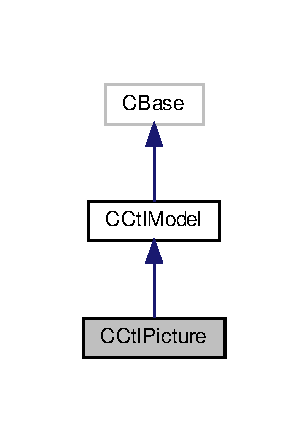
\includegraphics[width=148pt]{classCCtlPicture__inherit__graph}
\end{center}
\end{figure}


Collaboration diagram for C\+Ctl\+Picture\+:
\nopagebreak
\begin{figure}[H]
\begin{center}
\leavevmode
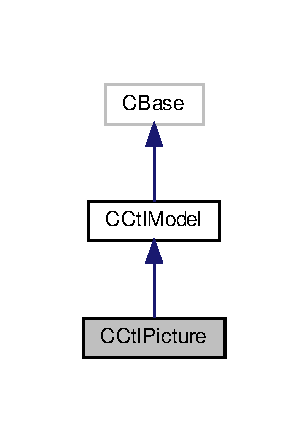
\includegraphics[width=148pt]{classCCtlPicture__coll__graph}
\end{center}
\end{figure}
\subsection*{Public Types}
\begin{DoxyCompactItemize}
\item 
\mbox{\Hypertarget{classCCtlPicture_ac613a207c19c1190c12302eda6b492b8}\label{classCCtlPicture_ac613a207c19c1190c12302eda6b492b8}} 
enum {\bfseries T\+Alignment} \{ {\bfseries E\+V\+Center} = 1, 
{\bfseries E\+V\+Top} = 2
 \}
\end{DoxyCompactItemize}
\subsection*{Public Member Functions}
\begin{DoxyCompactItemize}
\item 
\mbox{\Hypertarget{classCCtlPicture_ad59f0a33a23ec38be2b723d49b29c757}\label{classCCtlPicture_ad59f0a33a23ec38be2b723d49b29c757}} 
virtual \hyperlink{classCCtlModel}{C\+Ctl\+Model} $\ast$ {\bfseries Clone} ()
\item 
\mbox{\Hypertarget{classCCtlPicture_ae86c0d22494567c825c7a55a24b12a76}\label{classCCtlPicture_ae86c0d22494567c825c7a55a24b12a76}} 
virtual \hyperlink{classCCtlModel}{C\+Ctl\+Model} $\ast$ {\bfseries Clone3D} ()
\item 
\mbox{\Hypertarget{classCCtlPicture_a09d0d083303eeec4b0869cc5e98f9540}\label{classCCtlPicture_a09d0d083303eeec4b0869cc5e98f9540}} 
virtual void {\bfseries Draw} (C\+Window\+Gc \&gc, const T\+Rect $\ast$a\+Rect) const
\item 
\mbox{\Hypertarget{classCCtlPicture_af1a750feab4e7f7073c59eaaac6fe643}\label{classCCtlPicture_af1a750feab4e7f7073c59eaaac6fe643}} 
C\+Gul\+Icon $\ast$ {\bfseries Picture} ()
\item 
\mbox{\Hypertarget{classCCtlPicture_ab9acc69bb200deccfe03c5d132f55902}\label{classCCtlPicture_ab9acc69bb200deccfe03c5d132f55902}} 
void {\bfseries Set\+Picture} (C\+Gul\+Icon $\ast$a\+Gul\+Icon)
\item 
\mbox{\Hypertarget{classCCtlPicture_a047f1e2bf4cd6501f23fd7b3a551249e}\label{classCCtlPicture_a047f1e2bf4cd6501f23fd7b3a551249e}} 
void {\bfseries Set\+Alignment} (T\+Int a\+Alignment)
\item 
\mbox{\Hypertarget{classCCtlPicture_a6f503fb9691b8996fadf2a3c985641de}\label{classCCtlPicture_a6f503fb9691b8996fadf2a3c985641de}} 
void {\bfseries Set\+Bitmaps\+Owned\+Externally} (T\+Bool a\+Bitmaps\+Owned\+Externally)
\end{DoxyCompactItemize}
\subsection*{Static Public Member Functions}
\begin{DoxyCompactItemize}
\item 
\mbox{\Hypertarget{classCCtlPicture_ae5436e48137a6d653778ffc9e1f288ff}\label{classCCtlPicture_ae5436e48137a6d653778ffc9e1f288ff}} 
static \hyperlink{classCCtlPicture}{C\+Ctl\+Picture} $\ast$ {\bfseries NewL} (C\+Gul\+Icon $\ast$a\+Icon)
\item 
\mbox{\Hypertarget{classCCtlPicture_a4afce1123e686d0f3df6de6ca8cd44e7}\label{classCCtlPicture_a4afce1123e686d0f3df6de6ca8cd44e7}} 
static \hyperlink{classCCtlPicture}{C\+Ctl\+Picture} $\ast$ {\bfseries New\+LC} (C\+Gul\+Icon $\ast$a\+Icon)
\end{DoxyCompactItemize}


The documentation for this class was generated from the following files\+:\begin{DoxyCompactItemize}
\item 
/home/peter/work/github/\+Barba\+G\+U\+I/inc/\+Ctl/Ctl\+Picture.\+h\item 
/home/peter/work/github/\+Barba\+G\+U\+I/src/\+Ctl/Ctl\+Picture.\+cpp\end{DoxyCompactItemize}

\hypertarget{classCCtlRect}{}\section{C\+Ctl\+Rect Class Reference}
\label{classCCtlRect}\index{C\+Ctl\+Rect@{C\+Ctl\+Rect}}


Inheritance diagram for C\+Ctl\+Rect\+:
\nopagebreak
\begin{figure}[H]
\begin{center}
\leavevmode
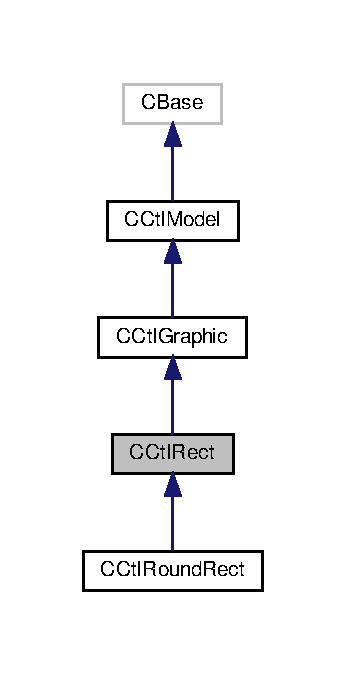
\includegraphics[width=166pt]{classCCtlRect__inherit__graph}
\end{center}
\end{figure}


Collaboration diagram for C\+Ctl\+Rect\+:
\nopagebreak
\begin{figure}[H]
\begin{center}
\leavevmode
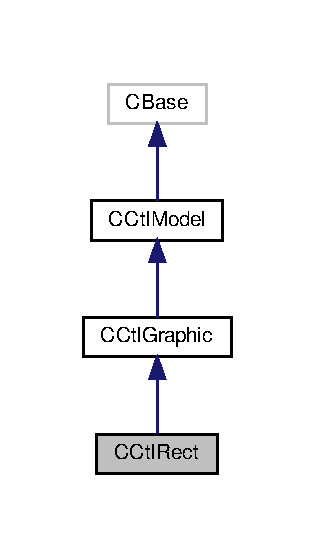
\includegraphics[width=151pt]{classCCtlRect__coll__graph}
\end{center}
\end{figure}
\subsection*{Public Member Functions}
\begin{DoxyCompactItemize}
\item 
\mbox{\Hypertarget{classCCtlRect_af2e9d6637c617c2e6f433645ca7767ac}\label{classCCtlRect_af2e9d6637c617c2e6f433645ca7767ac}} 
virtual \hyperlink{classCCtlModel}{C\+Ctl\+Model} $\ast$ {\bfseries Clone} ()
\item 
\mbox{\Hypertarget{classCCtlRect_af0e3e97cfcc25a913e940821267dea56}\label{classCCtlRect_af0e3e97cfcc25a913e940821267dea56}} 
virtual \hyperlink{classCCtlModel}{C\+Ctl\+Model} $\ast$ {\bfseries Clone3D} ()
\item 
\mbox{\Hypertarget{classCCtlRect_a75ff051c619c7e4e967548934c85fad1}\label{classCCtlRect_a75ff051c619c7e4e967548934c85fad1}} 
virtual void {\bfseries Draw} (C\+Window\+Gc \&gc, const T\+Rect $\ast$a\+Rect) const
\item 
\mbox{\Hypertarget{classCCtlRect_a70b13e08edc267da43dfbc1f29856db9}\label{classCCtlRect_a70b13e08edc267da43dfbc1f29856db9}} 
\hyperlink{classCCtlRect_a70b13e08edc267da43dfbc1f29856db9}{C\+Ctl\+Rect} (T\+Rgb a\+Pen\+Color)
\begin{DoxyCompactList}\small\item\em \hyperlink{classCCtlRect}{C\+Ctl\+Rect}. \end{DoxyCompactList}\item 
\mbox{\Hypertarget{classCCtlRect_ad666d07312d1fc2ec9cd1d28bde26ba5}\label{classCCtlRect_ad666d07312d1fc2ec9cd1d28bde26ba5}} 
void {\bfseries Set\+Brush\+Color} (T\+Rgb a\+Brush\+Color)
\item 
\mbox{\Hypertarget{classCCtlRect_a590ad7db1f3ddf9273f7bc544b1473be}\label{classCCtlRect_a590ad7db1f3ddf9273f7bc544b1473be}} 
void {\bfseries Set\+Brush\+Style} (T\+Int a\+Brush\+Style)
\item 
\mbox{\Hypertarget{classCCtlRect_a729abc05fd674a17b9142adffb11b4a1}\label{classCCtlRect_a729abc05fd674a17b9142adffb11b4a1}} 
void {\bfseries Set\+Pen\+Style} (T\+Int a\+Pen\+Style)
\item 
\mbox{\Hypertarget{classCCtlRect_a76c6edde142573cf406a1ece4cc8b261}\label{classCCtlRect_a76c6edde142573cf406a1ece4cc8b261}} 
void {\bfseries Set\+Pen\+Color} (T\+Rgb a\+Pen\+Color)
\item 
\mbox{\Hypertarget{classCCtlRect_a904b5b1a71326405abc594803318c5e2}\label{classCCtlRect_a904b5b1a71326405abc594803318c5e2}} 
void {\bfseries Set\+Pen\+Size} (T\+Size a\+Size)
\end{DoxyCompactItemize}
\subsection*{Protected Attributes}
\begin{DoxyCompactItemize}
\item 
\mbox{\Hypertarget{classCCtlRect_a10c0d7e6d949d086951b0cb5f91f3f43}\label{classCCtlRect_a10c0d7e6d949d086951b0cb5f91f3f43}} 
T\+Rgb {\bfseries i\+Brush\+Color}
\item 
\mbox{\Hypertarget{classCCtlRect_a1ef3da3994db751a7463c8d7b0b38736}\label{classCCtlRect_a1ef3da3994db751a7463c8d7b0b38736}} 
T\+Int {\bfseries i\+Brush\+Style}
\item 
\mbox{\Hypertarget{classCCtlRect_a2e0dccb3e579c7ab6041650f5d94773a}\label{classCCtlRect_a2e0dccb3e579c7ab6041650f5d94773a}} 
T\+Int {\bfseries i\+Pen\+Style}
\item 
\mbox{\Hypertarget{classCCtlRect_af31ea80a496344a97a174f578dbf0042}\label{classCCtlRect_af31ea80a496344a97a174f578dbf0042}} 
T\+Rgb {\bfseries i\+Pen\+Color}
\item 
\mbox{\Hypertarget{classCCtlRect_ae47ad0330838319d1c76d21c3bed61a9}\label{classCCtlRect_ae47ad0330838319d1c76d21c3bed61a9}} 
T\+Size {\bfseries i\+Pen\+Size}
\end{DoxyCompactItemize}
\subsection*{Additional Inherited Members}


The documentation for this class was generated from the following files\+:\begin{DoxyCompactItemize}
\item 
/home/peter/work/github/\+Barba\+G\+U\+I/inc/\+Ctl/Ctl\+Graphic.\+h\item 
/home/peter/work/github/\+Barba\+G\+U\+I/src/\+Ctl/Ctl\+Graphic.\+cpp\end{DoxyCompactItemize}

\hypertarget{classCCtlRoundRect}{}\section{C\+Ctl\+Round\+Rect Class Reference}
\label{classCCtlRoundRect}\index{C\+Ctl\+Round\+Rect@{C\+Ctl\+Round\+Rect}}


Inheritance diagram for C\+Ctl\+Round\+Rect\+:
\nopagebreak
\begin{figure}[H]
\begin{center}
\leavevmode
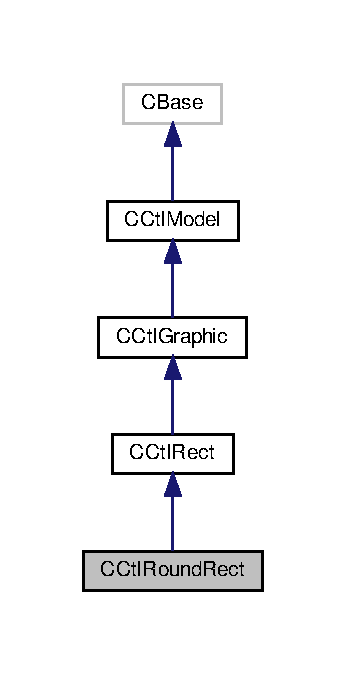
\includegraphics[width=166pt]{classCCtlRoundRect__inherit__graph}
\end{center}
\end{figure}


Collaboration diagram for C\+Ctl\+Round\+Rect\+:
\nopagebreak
\begin{figure}[H]
\begin{center}
\leavevmode
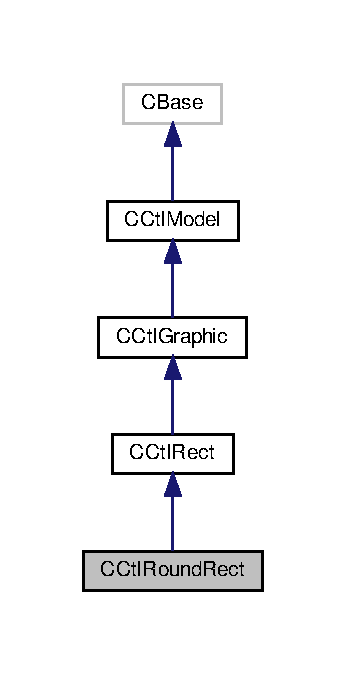
\includegraphics[width=166pt]{classCCtlRoundRect__coll__graph}
\end{center}
\end{figure}
\subsection*{Public Member Functions}
\begin{DoxyCompactItemize}
\item 
\mbox{\Hypertarget{classCCtlRoundRect_a3157984a6caeb5294c9cf978a9bf991e}\label{classCCtlRoundRect_a3157984a6caeb5294c9cf978a9bf991e}} 
virtual \hyperlink{classCCtlModel}{C\+Ctl\+Model} $\ast$ {\bfseries Clone} ()
\item 
\mbox{\Hypertarget{classCCtlRoundRect_a7db0f2b41845cbaa673d1c0342b494da}\label{classCCtlRoundRect_a7db0f2b41845cbaa673d1c0342b494da}} 
virtual \hyperlink{classCCtlModel}{C\+Ctl\+Model} $\ast$ {\bfseries Clone3D} ()
\item 
\mbox{\Hypertarget{classCCtlRoundRect_ac1e54eafbd2af874b0b845691e7beb3a}\label{classCCtlRoundRect_ac1e54eafbd2af874b0b845691e7beb3a}} 
virtual void {\bfseries Draw} (C\+Window\+Gc \&gc, const T\+Rect $\ast$a\+Rect) const
\item 
\mbox{\Hypertarget{classCCtlRoundRect_a14f57faf4eaf70818cbe9309a0d82109}\label{classCCtlRoundRect_a14f57faf4eaf70818cbe9309a0d82109}} 
\hyperlink{classCCtlRoundRect_a14f57faf4eaf70818cbe9309a0d82109}{C\+Ctl\+Round\+Rect} (T\+Rgb a\+Pen\+Color)
\begin{DoxyCompactList}\small\item\em \hyperlink{classCCtlRoundRect}{C\+Ctl\+Round\+Rect}. \end{DoxyCompactList}\item 
\mbox{\Hypertarget{classCCtlRoundRect_acbcfb1d6dc856ef8056cc8d60577efb9}\label{classCCtlRoundRect_acbcfb1d6dc856ef8056cc8d60577efb9}} 
void {\bfseries Set\+Corner\+Size} (T\+Size a\+Size)
\end{DoxyCompactItemize}
\subsection*{Additional Inherited Members}


The documentation for this class was generated from the following files\+:\begin{DoxyCompactItemize}
\item 
/home/peter/work/github/\+Barba\+G\+U\+I/inc/\+Ctl/Ctl\+Graphic.\+h\item 
/home/peter/work/github/\+Barba\+G\+U\+I/src/\+Ctl/Ctl\+Graphic.\+cpp\end{DoxyCompactItemize}

\hypertarget{classCCtlRow}{}\section{C\+Ctl\+Row Class Reference}
\label{classCCtlRow}\index{C\+Ctl\+Row@{C\+Ctl\+Row}}


Inheritance diagram for C\+Ctl\+Row\+:
\nopagebreak
\begin{figure}[H]
\begin{center}
\leavevmode
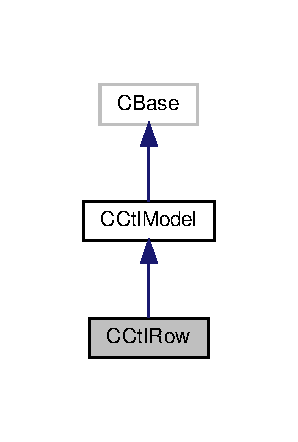
\includegraphics[width=143pt]{classCCtlRow__inherit__graph}
\end{center}
\end{figure}


Collaboration diagram for C\+Ctl\+Row\+:
\nopagebreak
\begin{figure}[H]
\begin{center}
\leavevmode
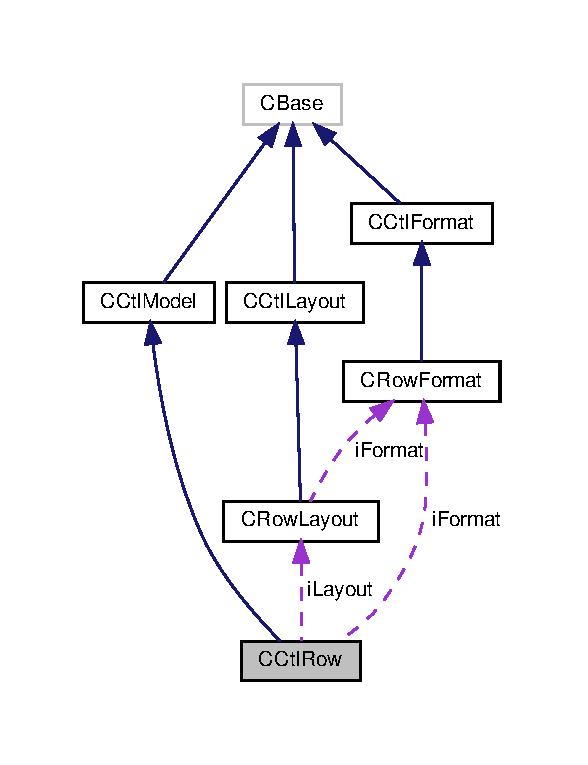
\includegraphics[width=282pt]{classCCtlRow__coll__graph}
\end{center}
\end{figure}
\subsection*{Public Member Functions}
\begin{DoxyCompactItemize}
\item 
\mbox{\Hypertarget{classCCtlRow_a6ca919a0199728ecc074bc1535e66d21}\label{classCCtlRow_a6ca919a0199728ecc074bc1535e66d21}} 
virtual void {\bfseries Add} (\hyperlink{classCCtlModel}{C\+Ctl\+Model} $\ast$a\+Ctl\+Model)
\item 
\mbox{\Hypertarget{classCCtlRow_ae8321a5204f1ccd60adf17b955ff9655}\label{classCCtlRow_ae8321a5204f1ccd60adf17b955ff9655}} 
virtual void {\bfseries Remove} (T\+Int an\+Index)
\item 
\mbox{\Hypertarget{classCCtlRow_a20d7f8cc1a807a0007c518fcc64601a4}\label{classCCtlRow_a20d7f8cc1a807a0007c518fcc64601a4}} 
virtual T\+Int {\bfseries Insert} (\hyperlink{classCCtlModel}{C\+Ctl\+Model} $\ast$a\+Ctl\+Model, T\+Int a\+Pos)
\item 
\mbox{\Hypertarget{classCCtlRow_a4c73c3acc51e3a77307f5dfed79b097d}\label{classCCtlRow_a4c73c3acc51e3a77307f5dfed79b097d}} 
virtual void {\bfseries Reset} ()
\item 
\mbox{\Hypertarget{classCCtlRow_a1787fe65c0cd77a6644a7d5a4a9b3eb3}\label{classCCtlRow_a1787fe65c0cd77a6644a7d5a4a9b3eb3}} 
virtual T\+Int {\bfseries Count} ()
\item 
\mbox{\Hypertarget{classCCtlRow_a7f550d876fe41f3f0cf0e11c9fe8cd9d}\label{classCCtlRow_a7f550d876fe41f3f0cf0e11c9fe8cd9d}} 
virtual void {\bfseries Draw} (C\+Window\+Gc \&gc, const T\+Rect $\ast$a\+Rect) const
\item 
\mbox{\Hypertarget{classCCtlRow_a254b1246d84231b15fddd19a0d265dc9}\label{classCCtlRow_a254b1246d84231b15fddd19a0d265dc9}} 
virtual void {\bfseries Make\+Visible} (T\+Bool a\+Visible)
\item 
\mbox{\Hypertarget{classCCtlRow_a26a84421ba99cb16e657ca67628201fc}\label{classCCtlRow_a26a84421ba99cb16e657ca67628201fc}} 
virtual \hyperlink{classCCtlModel}{C\+Ctl\+Model} $\ast$ {\bfseries At} (T\+Int a\+Index)
\item 
\mbox{\Hypertarget{classCCtlRow_aa072887b40bc71bc218686df92e04c20}\label{classCCtlRow_aa072887b40bc71bc218686df92e04c20}} 
virtual \hyperlink{classCCtlModel}{C\+Ctl\+Model} $\ast$ {\bfseries Clone} ()
\item 
\mbox{\Hypertarget{classCCtlRow_ab7d8b6ee27f84d0e074e93f47386a7aa}\label{classCCtlRow_ab7d8b6ee27f84d0e074e93f47386a7aa}} 
virtual \hyperlink{classCCtlModel}{C\+Ctl\+Model} $\ast$ {\bfseries Clone3D} ()
\item 
\mbox{\Hypertarget{classCCtlRow_a663a9568d7aee3243d4d50d02f52aff2}\label{classCCtlRow_a663a9568d7aee3243d4d50d02f52aff2}} 
virtual T\+Rect $\ast$ {\bfseries Rect} () const
\item 
\mbox{\Hypertarget{classCCtlRow_a36a8453bd1ff2a6edc70b7377e2478ba}\label{classCCtlRow_a36a8453bd1ff2a6edc70b7377e2478ba}} 
void {\bfseries Set\+Rect} (const T\+Rect \&a\+Rect)
\item 
\mbox{\Hypertarget{classCCtlRow_a2f92c5996bf38f3b564d62476e52324a}\label{classCCtlRow_a2f92c5996bf38f3b564d62476e52324a}} 
void {\bfseries Set\+View\+Rect} (const T\+Rect \&a\+Rect)
\item 
\mbox{\Hypertarget{classCCtlRow_a619a8ac5af3be217d424e6d9dbb4ad22}\label{classCCtlRow_a619a8ac5af3be217d424e6d9dbb4ad22}} 
const T\+Rect \& {\bfseries View\+Rect} () const
\item 
\mbox{\Hypertarget{classCCtlRow_a533cdd6ffbd0aaa8ae8d09f5f7ee7895}\label{classCCtlRow_a533cdd6ffbd0aaa8ae8d09f5f7ee7895}} 
void {\bfseries Set\+Layout} (\hyperlink{classCRowLayout}{C\+Row\+Layout} $\ast$a\+Layout)
\item 
\mbox{\Hypertarget{classCCtlRow_a006578f546a71f2d1faed274abfef3bb}\label{classCCtlRow_a006578f546a71f2d1faed274abfef3bb}} 
\hyperlink{classCRowFormat}{C\+Row\+Format} $\ast$ {\bfseries Format} ()
\item 
\mbox{\Hypertarget{classCCtlRow_a99a44bff64b591b39908c719b729f088}\label{classCCtlRow_a99a44bff64b591b39908c719b729f088}} 
void {\bfseries Set\+Format} (\hyperlink{classCRowFormat}{C\+Row\+Format} $\ast$a\+Format)
\item 
\mbox{\Hypertarget{classCCtlRow_a92981b941bd509ffc9fdf2421d96f2ab}\label{classCCtlRow_a92981b941bd509ffc9fdf2421d96f2ab}} 
T\+Int {\bfseries Get\+Selection} (const T\+Point \&a\+Point, T\+Bool a\+Is\+Top\+First=E\+True)
\end{DoxyCompactItemize}
\subsection*{Static Public Member Functions}
\begin{DoxyCompactItemize}
\item 
\mbox{\Hypertarget{classCCtlRow_ace17a35f5a1f9c76e24633e4c78de51f}\label{classCCtlRow_ace17a35f5a1f9c76e24633e4c78de51f}} 
static \hyperlink{classCCtlRow}{C\+Ctl\+Row} $\ast$ {\bfseries NewL} ()
\item 
\mbox{\Hypertarget{classCCtlRow_a4af427a3a325d3cd389f83d160340b64}\label{classCCtlRow_a4af427a3a325d3cd389f83d160340b64}} 
static \hyperlink{classCCtlRow}{C\+Ctl\+Row} $\ast$ {\bfseries New\+LC} ()
\end{DoxyCompactItemize}
\subsection*{Protected Member Functions}
\begin{DoxyCompactItemize}
\item 
\mbox{\Hypertarget{classCCtlRow_a7274b925917b848111a8584b110d0396}\label{classCCtlRow_a7274b925917b848111a8584b110d0396}} 
void {\bfseries ConstructL} ()
\end{DoxyCompactItemize}
\subsection*{Protected Attributes}
\begin{DoxyCompactItemize}
\item 
\mbox{\Hypertarget{classCCtlRow_a563f72aff84e4ad4d77ed66217457ac5}\label{classCCtlRow_a563f72aff84e4ad4d77ed66217457ac5}} 
R\+Pointer\+Array$<$ \hyperlink{classCCtlModel}{C\+Ctl\+Model} $>$ $\ast$ {\bfseries i\+Components}
\item 
\mbox{\Hypertarget{classCCtlRow_a4ae1bb05d6eb1c1868730875b8e3c8b4}\label{classCCtlRow_a4ae1bb05d6eb1c1868730875b8e3c8b4}} 
\hyperlink{classCRowLayout}{C\+Row\+Layout} $\ast$ {\bfseries i\+Layout}
\item 
\mbox{\Hypertarget{classCCtlRow_a5a23983f61f139bcc58eba003e590dba}\label{classCCtlRow_a5a23983f61f139bcc58eba003e590dba}} 
T\+Bool {\bfseries i\+Visible}
\item 
\mbox{\Hypertarget{classCCtlRow_ad2274ce7ce1a5a14717b1d773fa5bc08}\label{classCCtlRow_ad2274ce7ce1a5a14717b1d773fa5bc08}} 
\hyperlink{classCRowFormat}{C\+Row\+Format} $\ast$ {\bfseries i\+Format}
\end{DoxyCompactItemize}


The documentation for this class was generated from the following files\+:\begin{DoxyCompactItemize}
\item 
/home/peter/work/github/\+Barba\+G\+U\+I/inc/\+Ctl/Ctl\+Row.\+h\item 
/home/peter/work/github/\+Barba\+G\+U\+I/src/\+Ctl/Ctl\+Row.\+cpp\end{DoxyCompactItemize}

\hypertarget{classCCtlText}{}\section{C\+Ctl\+Text Class Reference}
\label{classCCtlText}\index{C\+Ctl\+Text@{C\+Ctl\+Text}}


Inheritance diagram for C\+Ctl\+Text\+:
\nopagebreak
\begin{figure}[H]
\begin{center}
\leavevmode
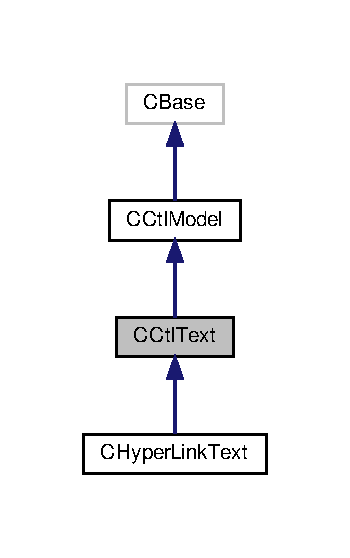
\includegraphics[width=168pt]{classCCtlText__inherit__graph}
\end{center}
\end{figure}


Collaboration diagram for C\+Ctl\+Text\+:
\nopagebreak
\begin{figure}[H]
\begin{center}
\leavevmode
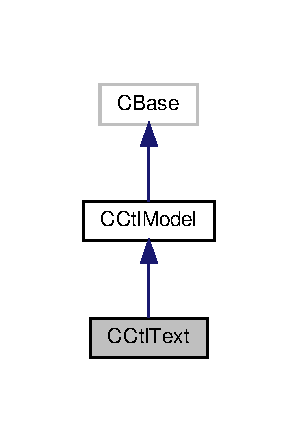
\includegraphics[width=143pt]{classCCtlText__coll__graph}
\end{center}
\end{figure}
\subsection*{Public Member Functions}
\begin{DoxyCompactItemize}
\item 
\mbox{\Hypertarget{classCCtlText_a6f9c29066dff07c8231ef6e12d32e2ec}\label{classCCtlText_a6f9c29066dff07c8231ef6e12d32e2ec}} 
virtual \hyperlink{classCCtlModel}{C\+Ctl\+Model} $\ast$ {\bfseries Clone} ()
\item 
\mbox{\Hypertarget{classCCtlText_a2cdb8b10f87f3f470c97801129931fd6}\label{classCCtlText_a2cdb8b10f87f3f470c97801129931fd6}} 
virtual \hyperlink{classCCtlModel}{C\+Ctl\+Model} $\ast$ {\bfseries Clone3D} ()
\item 
\mbox{\Hypertarget{classCCtlText_a63d72ea3f9b9bafea7cf011d15e87bc4}\label{classCCtlText_a63d72ea3f9b9bafea7cf011d15e87bc4}} 
virtual void {\bfseries Draw} (C\+Window\+Gc \&gc, const T\+Rect $\ast$a\+Rect) const
\item 
\mbox{\Hypertarget{classCCtlText_a3fa7aa2abdcef26bee1b1f6612c5e7a6}\label{classCCtlText_a3fa7aa2abdcef26bee1b1f6612c5e7a6}} 
void {\bfseries Get\+Text} (T\+PtrC \&a\+Text)
\item 
\mbox{\Hypertarget{classCCtlText_ad59eebb9e02b580efc129c7bbfe79750}\label{classCCtlText_ad59eebb9e02b580efc129c7bbfe79750}} 
void {\bfseries Set\+Text} (const T\+DesC \&a\+Text)
\end{DoxyCompactItemize}
\subsection*{Static Public Member Functions}
\begin{DoxyCompactItemize}
\item 
\mbox{\Hypertarget{classCCtlText_a13a1f4c0a0d1e433e61603dbde1c84e1}\label{classCCtlText_a13a1f4c0a0d1e433e61603dbde1c84e1}} 
static \hyperlink{classCCtlText}{C\+Ctl\+Text} $\ast$ {\bfseries NewL} (const T\+DesC \&a\+Text, T\+Int a\+Style\+Index)
\item 
\mbox{\Hypertarget{classCCtlText_a634f0346de9b9ebcf757f6ba8816ede5}\label{classCCtlText_a634f0346de9b9ebcf757f6ba8816ede5}} 
static \hyperlink{classCCtlText}{C\+Ctl\+Text} $\ast$ {\bfseries New\+LC} (const T\+DesC \&a\+Text, T\+Int a\+Style\+Index)
\end{DoxyCompactItemize}
\subsection*{Protected Member Functions}
\begin{DoxyCompactItemize}
\item 
\mbox{\Hypertarget{classCCtlText_ad74d1e3b0492b2175bc756d661daa025}\label{classCCtlText_ad74d1e3b0492b2175bc756d661daa025}} 
void {\bfseries ConstructL} (const T\+DesC \&a\+Text, T\+Int a\+Style\+Index)
\end{DoxyCompactItemize}
\subsection*{Protected Attributes}
\begin{DoxyCompactItemize}
\item 
\mbox{\Hypertarget{classCCtlText_a3c031dd75b9448dee44a671349a6a175}\label{classCCtlText_a3c031dd75b9448dee44a671349a6a175}} 
R\+Buf {\bfseries i\+Text}
\item 
\mbox{\Hypertarget{classCCtlText_a1840cfe7b9336e46c69ee0a7b330fd79}\label{classCCtlText_a1840cfe7b9336e46c69ee0a7b330fd79}} 
T\+Int {\bfseries i\+Style\+Index}
\end{DoxyCompactItemize}


The documentation for this class was generated from the following files\+:\begin{DoxyCompactItemize}
\item 
/home/peter/work/github/\+Barba\+G\+U\+I/inc/\+Ctl/Ctl\+Text.\+h\item 
/home/peter/work/github/\+Barba\+G\+U\+I/src/\+Ctl/Ctl\+Text.\+cpp\end{DoxyCompactItemize}

\hypertarget{classCDeceleratedMotion}{}\section{C\+Decelerated\+Motion Class Reference}
\label{classCDeceleratedMotion}\index{C\+Decelerated\+Motion@{C\+Decelerated\+Motion}}


Inheritance diagram for C\+Decelerated\+Motion\+:
\nopagebreak
\begin{figure}[H]
\begin{center}
\leavevmode
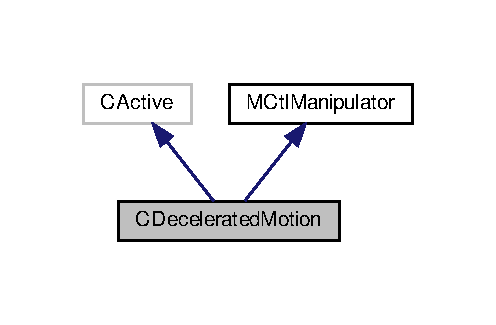
\includegraphics[width=238pt]{classCDeceleratedMotion__inherit__graph}
\end{center}
\end{figure}


Collaboration diagram for C\+Decelerated\+Motion\+:
\nopagebreak
\begin{figure}[H]
\begin{center}
\leavevmode
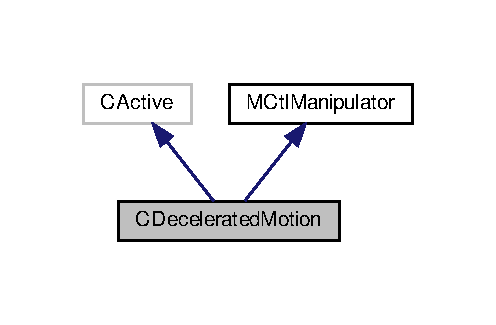
\includegraphics[width=238pt]{classCDeceleratedMotion__coll__graph}
\end{center}
\end{figure}
\subsection*{Public Member Functions}
\begin{DoxyCompactItemize}
\item 
\mbox{\Hypertarget{classCDeceleratedMotion_a1bc6987d63b48780c9ef93c88eae5530}\label{classCDeceleratedMotion_a1bc6987d63b48780c9ef93c88eae5530}} 
virtual void {\bfseries Handle\+Pointer\+EventL} (const T\+Pointer\+Event \&a\+Pointer\+Event)
\item 
\mbox{\Hypertarget{classCDeceleratedMotion_a8b11240612fdb78f9e3d202a64368b42}\label{classCDeceleratedMotion_a8b11240612fdb78f9e3d202a64368b42}} 
void {\bfseries Start\+Move} ()
\item 
\mbox{\Hypertarget{classCDeceleratedMotion_a2b4c06a772988cdb40b62415739f10f5}\label{classCDeceleratedMotion_a2b4c06a772988cdb40b62415739f10f5}} 
void {\bfseries Set\+Down\+Point} (const T\+Point \&a\+Point)
\item 
\mbox{\Hypertarget{classCDeceleratedMotion_affc8b87af909f3b7d337981e3e5f2714}\label{classCDeceleratedMotion_affc8b87af909f3b7d337981e3e5f2714}} 
void {\bfseries Set\+Up\+Point} (const T\+Point \&a\+Point)
\end{DoxyCompactItemize}
\subsection*{Static Public Member Functions}
\begin{DoxyCompactItemize}
\item 
static \hyperlink{classCDeceleratedMotion}{C\+Decelerated\+Motion} $\ast$ \hyperlink{classCDeceleratedMotion_afe86cb77999ad4f58a4e555208c1a1f0}{NewL} (\hyperlink{classCCtlColumn}{C\+Ctl\+Column} $\ast$a\+Model, C\+Video\+List\+Ctl $\ast$a\+View)
\begin{DoxyCompactList}\small\item\em \hyperlink{classCDelManipulator}{C\+Del\+Manipulator}. \end{DoxyCompactList}\item 
\mbox{\Hypertarget{classCDeceleratedMotion_a29adc2f04f18bfca6ec676746cae3872}\label{classCDeceleratedMotion_a29adc2f04f18bfca6ec676746cae3872}} 
static \hyperlink{classCDeceleratedMotion}{C\+Decelerated\+Motion} $\ast$ {\bfseries New\+LC} (\hyperlink{classCCtlColumn}{C\+Ctl\+Column} $\ast$a\+Model, C\+Video\+List\+Ctl $\ast$a\+View)
\end{DoxyCompactItemize}
\subsection*{Protected Types}
\begin{DoxyCompactItemize}
\item 
\mbox{\Hypertarget{classCDeceleratedMotion_a7499e52650dbbe1322a271fadcf9663c}\label{classCDeceleratedMotion_a7499e52650dbbe1322a271fadcf9663c}} 
enum {\bfseries T\+Motion\+State} \{ \newline
{\bfseries K\+Ready\+Move}, 
{\bfseries K\+Moving}, 
{\bfseries K\+Moved}, 
{\bfseries K\+Recovering}, 
\newline
{\bfseries K\+Recovered}
 \}
\end{DoxyCompactItemize}
\subsection*{Protected Member Functions}
\begin{DoxyCompactItemize}
\item 
\mbox{\Hypertarget{classCDeceleratedMotion_aa7c139e2ecade795a8df53b6d01b1e5b}\label{classCDeceleratedMotion_aa7c139e2ecade795a8df53b6d01b1e5b}} 
{\bfseries C\+Decelerated\+Motion} (\hyperlink{classCCtlColumn}{C\+Ctl\+Column} $\ast$a\+Model, C\+Video\+List\+Ctl $\ast$a\+View)
\item 
\mbox{\Hypertarget{classCDeceleratedMotion_a78ae777217ce1a6f54e64f7c4a855d9f}\label{classCDeceleratedMotion_a78ae777217ce1a6f54e64f7c4a855d9f}} 
void {\bfseries ConstructL} ()
\item 
\mbox{\Hypertarget{classCDeceleratedMotion_a2d36daaec92cd6f34af5a5286648c48d}\label{classCDeceleratedMotion_a2d36daaec92cd6f34af5a5286648c48d}} 
virtual void {\bfseries RunL} ()
\item 
\mbox{\Hypertarget{classCDeceleratedMotion_ae6292874608551ec8caa5cc4a9fb6a75}\label{classCDeceleratedMotion_ae6292874608551ec8caa5cc4a9fb6a75}} 
virtual void {\bfseries Do\+Cancel} ()
\end{DoxyCompactItemize}
\subsection*{Additional Inherited Members}


\subsection{Member Function Documentation}
\mbox{\Hypertarget{classCDeceleratedMotion_afe86cb77999ad4f58a4e555208c1a1f0}\label{classCDeceleratedMotion_afe86cb77999ad4f58a4e555208c1a1f0}} 
\index{C\+Decelerated\+Motion@{C\+Decelerated\+Motion}!NewL@{NewL}}
\index{NewL@{NewL}!C\+Decelerated\+Motion@{C\+Decelerated\+Motion}}
\subsubsection{\texorpdfstring{New\+L()}{NewL()}}
{\footnotesize\ttfamily \hyperlink{classCDeceleratedMotion}{C\+Decelerated\+Motion} $\ast$ C\+Decelerated\+Motion\+::\+NewL (\begin{DoxyParamCaption}\item[{\hyperlink{classCCtlColumn}{C\+Ctl\+Column} $\ast$}]{a\+Model,  }\item[{C\+Video\+List\+Ctl $\ast$}]{a\+View }\end{DoxyParamCaption})\hspace{0.3cm}{\ttfamily [static]}}



\hyperlink{classCDelManipulator}{C\+Del\+Manipulator}. 

\hyperlink{classCDeceleratedMotion}{C\+Decelerated\+Motion} 

The documentation for this class was generated from the following files\+:\begin{DoxyCompactItemize}
\item 
/home/peter/work/github/\+Barba\+G\+U\+I/inc/\+Ctl/ctlmanipulator.\+h\item 
/home/peter/work/github/\+Barba\+G\+U\+I/src/\+Ctl/Ctl\+Manipulator.\+cpp\end{DoxyCompactItemize}

\hypertarget{classCDelManipulator}{}\section{C\+Del\+Manipulator Class Reference}
\label{classCDelManipulator}\index{C\+Del\+Manipulator@{C\+Del\+Manipulator}}


Inheritance diagram for C\+Del\+Manipulator\+:
\nopagebreak
\begin{figure}[H]
\begin{center}
\leavevmode
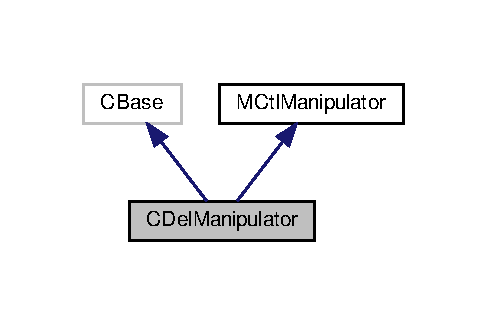
\includegraphics[width=234pt]{classCDelManipulator__inherit__graph}
\end{center}
\end{figure}


Collaboration diagram for C\+Del\+Manipulator\+:
\nopagebreak
\begin{figure}[H]
\begin{center}
\leavevmode
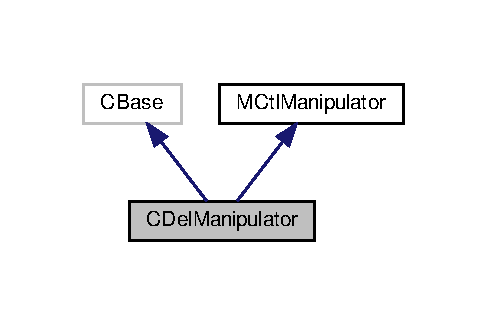
\includegraphics[width=234pt]{classCDelManipulator__coll__graph}
\end{center}
\end{figure}
\subsection*{Public Member Functions}
\begin{DoxyCompactItemize}
\item 
\mbox{\Hypertarget{classCDelManipulator_acb37452f6ac4ee3cc7b6d604cfaa02a0}\label{classCDelManipulator_acb37452f6ac4ee3cc7b6d604cfaa02a0}} 
{\bfseries C\+Del\+Manipulator} (C\+Y\+K\+Column $\ast$a\+Model, C\+Preference\+List\+Ctl $\ast$a\+View)
\item 
\mbox{\Hypertarget{classCDelManipulator_a69993964935447727ff7b048891f758f}\label{classCDelManipulator_a69993964935447727ff7b048891f758f}} 
virtual void {\bfseries Handle\+Pointer\+EventL} (const T\+Pointer\+Event \&a\+Pointer\+Event)
\end{DoxyCompactItemize}
\subsection*{Additional Inherited Members}


The documentation for this class was generated from the following file\+:\begin{DoxyCompactItemize}
\item 
/home/peter/work/github/\+Barba\+G\+U\+I/inc/\+Ctl/ctlmanipulator.\+h\end{DoxyCompactItemize}

\hypertarget{classCDragManipulator}{}\section{C\+Drag\+Manipulator Class Reference}
\label{classCDragManipulator}\index{C\+Drag\+Manipulator@{C\+Drag\+Manipulator}}


Inheritance diagram for C\+Drag\+Manipulator\+:
\nopagebreak
\begin{figure}[H]
\begin{center}
\leavevmode
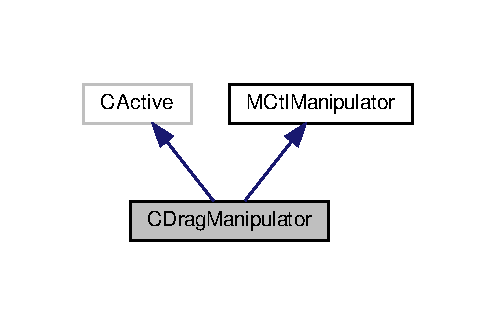
\includegraphics[width=238pt]{classCDragManipulator__inherit__graph}
\end{center}
\end{figure}


Collaboration diagram for C\+Drag\+Manipulator\+:
\nopagebreak
\begin{figure}[H]
\begin{center}
\leavevmode
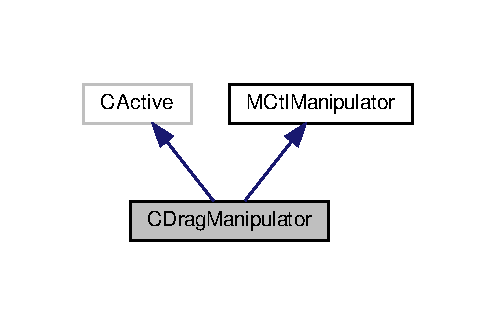
\includegraphics[width=238pt]{classCDragManipulator__coll__graph}
\end{center}
\end{figure}
\subsection*{Public Types}
\begin{DoxyCompactItemize}
\item 
\mbox{\Hypertarget{classCDragManipulator_a23f98fce4819a2420775120994cf4ebb}\label{classCDragManipulator_a23f98fce4819a2420775120994cf4ebb}} 
enum {\bfseries T\+Scroll\+State} \{ {\bfseries E\+Ready}, 
{\bfseries E\+Scroll\+Up}, 
{\bfseries E\+Scroll\+Down}
 \}
\end{DoxyCompactItemize}
\subsection*{Public Member Functions}
\begin{DoxyCompactItemize}
\item 
\mbox{\Hypertarget{classCDragManipulator_a7d2c7d5bb799254782475e4e2e057c0c}\label{classCDragManipulator_a7d2c7d5bb799254782475e4e2e057c0c}} 
void {\bfseries Start\+Exchange} ()
\item 
\mbox{\Hypertarget{classCDragManipulator_acb55dadea424e7cdb528abbc09431d6a}\label{classCDragManipulator_acb55dadea424e7cdb528abbc09431d6a}} 
virtual void {\bfseries Handle\+Pointer\+EventL} (const T\+Pointer\+Event \&a\+Pointer\+Event)
\item 
\mbox{\Hypertarget{classCDragManipulator_a84a39ea56423e47958b4d4568f6f4b94}\label{classCDragManipulator_a84a39ea56423e47958b4d4568f6f4b94}} 
virtual void {\bfseries Draw} (C\+Window\+Gc \&gc) const
\end{DoxyCompactItemize}
\subsection*{Static Public Member Functions}
\begin{DoxyCompactItemize}
\item 
\mbox{\Hypertarget{classCDragManipulator_a6ba4590ac279eada6a7e4e12c1398171}\label{classCDragManipulator_a6ba4590ac279eada6a7e4e12c1398171}} 
static \hyperlink{classCDragManipulator}{C\+Drag\+Manipulator} $\ast$ {\bfseries NewL} (C\+Y\+K\+Column $\ast$a\+Model, C\+Preference\+List\+Ctl $\ast$a\+View)
\item 
\mbox{\Hypertarget{classCDragManipulator_acf6b8ce97de139a0673884aa3529eda3}\label{classCDragManipulator_acf6b8ce97de139a0673884aa3529eda3}} 
static \hyperlink{classCDragManipulator}{C\+Drag\+Manipulator} $\ast$ {\bfseries New\+LC} (C\+Y\+K\+Column $\ast$a\+Model, C\+Preference\+List\+Ctl $\ast$a\+View)
\end{DoxyCompactItemize}
\subsection*{Additional Inherited Members}


The documentation for this class was generated from the following file\+:\begin{DoxyCompactItemize}
\item 
/home/peter/work/github/\+Barba\+G\+U\+I/inc/\+Ctl/ctlmanipulator.\+h\end{DoxyCompactItemize}

\hypertarget{classCDragManipulator2}{}\section{C\+Drag\+Manipulator2 Class Reference}
\label{classCDragManipulator2}\index{C\+Drag\+Manipulator2@{C\+Drag\+Manipulator2}}


Inheritance diagram for C\+Drag\+Manipulator2\+:
\nopagebreak
\begin{figure}[H]
\begin{center}
\leavevmode
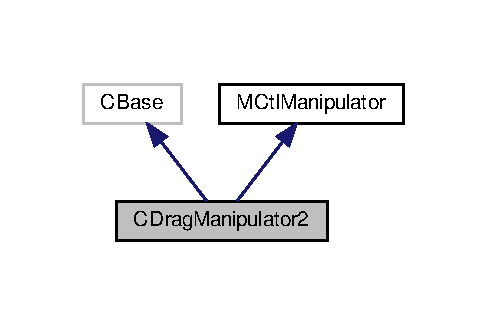
\includegraphics[width=234pt]{classCDragManipulator2__inherit__graph}
\end{center}
\end{figure}


Collaboration diagram for C\+Drag\+Manipulator2\+:
\nopagebreak
\begin{figure}[H]
\begin{center}
\leavevmode
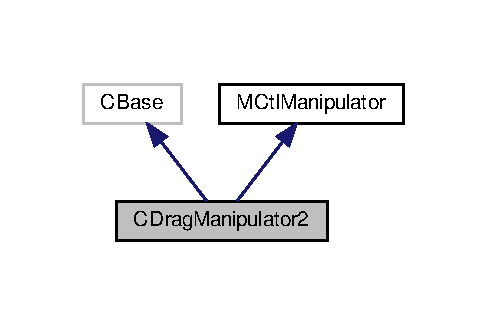
\includegraphics[width=234pt]{classCDragManipulator2__coll__graph}
\end{center}
\end{figure}
\subsection*{Public Member Functions}
\begin{DoxyCompactItemize}
\item 
\mbox{\Hypertarget{classCDragManipulator2_a7de95d6531395a969562c3ae81b050b4}\label{classCDragManipulator2_a7de95d6531395a969562c3ae81b050b4}} 
{\bfseries C\+Drag\+Manipulator2} (\hyperlink{classCCtlColumn}{C\+Ctl\+Column} $\ast$a\+Model, C\+Preference\+List\+Ctl $\ast$a\+View)
\item 
\mbox{\Hypertarget{classCDragManipulator2_a13effd7ec990464d7b1d4eff7b2ce3de}\label{classCDragManipulator2_a13effd7ec990464d7b1d4eff7b2ce3de}} 
virtual void {\bfseries Handle\+Pointer\+EventL} (const T\+Pointer\+Event \&a\+Pointer\+Event)
\item 
\mbox{\Hypertarget{classCDragManipulator2_a4b12e62a7bb018bb2411a6fc51ca2d6f}\label{classCDragManipulator2_a4b12e62a7bb018bb2411a6fc51ca2d6f}} 
virtual void {\bfseries Draw} (C\+Window\+Gc \&gc) const
\end{DoxyCompactItemize}
\subsection*{Additional Inherited Members}


The documentation for this class was generated from the following file\+:\begin{DoxyCompactItemize}
\item 
/home/peter/work/github/\+Barba\+G\+U\+I/inc/\+Ctl/ctlmanipulator.\+h\end{DoxyCompactItemize}

\hypertarget{classCHyperLinkText}{}\section{C\+Hyper\+Link\+Text Class Reference}
\label{classCHyperLinkText}\index{C\+Hyper\+Link\+Text@{C\+Hyper\+Link\+Text}}


Inheritance diagram for C\+Hyper\+Link\+Text\+:
\nopagebreak
\begin{figure}[H]
\begin{center}
\leavevmode
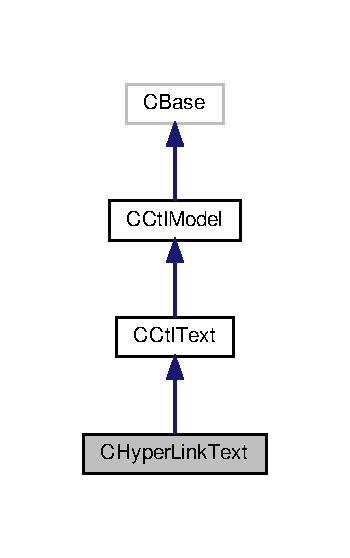
\includegraphics[width=168pt]{classCHyperLinkText__inherit__graph}
\end{center}
\end{figure}


Collaboration diagram for C\+Hyper\+Link\+Text\+:
\nopagebreak
\begin{figure}[H]
\begin{center}
\leavevmode
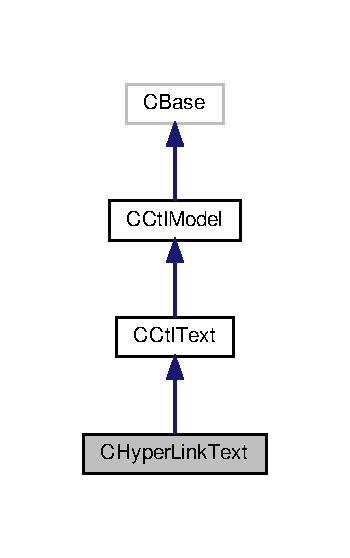
\includegraphics[width=168pt]{classCHyperLinkText__coll__graph}
\end{center}
\end{figure}
\subsection*{Public Types}
\begin{DoxyCompactItemize}
\item 
\mbox{\Hypertarget{classCHyperLinkText_acb95b4e70f69fb747810e9cd01be901f}\label{classCHyperLinkText_acb95b4e70f69fb747810e9cd01be901f}} 
enum \{ {\bfseries E\+Select\+None}, 
{\bfseries E\+Selected}
 \}
\item 
\mbox{\Hypertarget{classCHyperLinkText_a7bfc3eb05cd35e50d53dd8de137a9292}\label{classCHyperLinkText_a7bfc3eb05cd35e50d53dd8de137a9292}} 
enum {\bfseries T\+Alignment} \{ {\bfseries E\+H\+Center} = 1, 
{\bfseries E\+H\+Left} = 2
 \}
\end{DoxyCompactItemize}
\subsection*{Public Member Functions}
\begin{DoxyCompactItemize}
\item 
\mbox{\Hypertarget{classCHyperLinkText_a3089595917ab676ed5de18d67b056f3a}\label{classCHyperLinkText_a3089595917ab676ed5de18d67b056f3a}} 
virtual void {\bfseries Draw} (C\+Window\+Gc \&gc, const T\+Rect $\ast$a\+Rect) const
\item 
\mbox{\Hypertarget{classCHyperLinkText_accadc226d397931459d2319bc4f785a5}\label{classCHyperLinkText_accadc226d397931459d2319bc4f785a5}} 
void {\bfseries Set\+State} (T\+Int a\+State)
\item 
\mbox{\Hypertarget{classCHyperLinkText_a7012fb7b98d5957b70579f0a52bed366}\label{classCHyperLinkText_a7012fb7b98d5957b70579f0a52bed366}} 
T\+Int {\bfseries State} ()
\item 
\mbox{\Hypertarget{classCHyperLinkText_a32e3137efd3ac6fbaea1485a6aa71368}\label{classCHyperLinkText_a32e3137efd3ac6fbaea1485a6aa71368}} 
void {\bfseries Set\+Data} (H\+BufC $\ast$a\+Data)
\item 
\mbox{\Hypertarget{classCHyperLinkText_a727abd845e0bd95b8cbcf60d1eecd401}\label{classCHyperLinkText_a727abd845e0bd95b8cbcf60d1eecd401}} 
H\+BufC $\ast$ {\bfseries Data} ()
\item 
\mbox{\Hypertarget{classCHyperLinkText_a8ba2a5d24895587c3b6f4009e3f9c8f2}\label{classCHyperLinkText_a8ba2a5d24895587c3b6f4009e3f9c8f2}} 
void {\bfseries Set\+Alignment} (T\+Int a\+Alignment)
\end{DoxyCompactItemize}
\subsection*{Static Public Member Functions}
\begin{DoxyCompactItemize}
\item 
\mbox{\Hypertarget{classCHyperLinkText_a1a4039890d11d88831bf7bb86efbe2b0}\label{classCHyperLinkText_a1a4039890d11d88831bf7bb86efbe2b0}} 
static \hyperlink{classCHyperLinkText}{C\+Hyper\+Link\+Text} $\ast$ {\bfseries NewL} (const T\+DesC \&a\+Text, T\+Int a\+Style\+Index, T\+Int a\+Clicked\+Style\+Index)
\item 
\mbox{\Hypertarget{classCHyperLinkText_aad53389ae36964268e601a33c1576c38}\label{classCHyperLinkText_aad53389ae36964268e601a33c1576c38}} 
static \hyperlink{classCHyperLinkText}{C\+Hyper\+Link\+Text} $\ast$ {\bfseries New\+LC} (const T\+DesC \&a\+Text, T\+Int a\+Style\+Index, T\+Int a\+Clicked\+Style\+Index)
\end{DoxyCompactItemize}
\subsection*{Additional Inherited Members}


The documentation for this class was generated from the following files\+:\begin{DoxyCompactItemize}
\item 
/home/peter/work/github/\+Barba\+G\+U\+I/inc/\+Ctl/Hyper\+Link\+Text.\+h\item 
/home/peter/work/github/\+Barba\+G\+U\+I/src/\+Ctl/Hyper\+Link\+Text.\+cpp\end{DoxyCompactItemize}

\hypertarget{classCItemSelector}{}\section{C\+Item\+Selector Class Reference}
\label{classCItemSelector}\index{C\+Item\+Selector@{C\+Item\+Selector}}


Inheritance diagram for C\+Item\+Selector\+:
\nopagebreak
\begin{figure}[H]
\begin{center}
\leavevmode
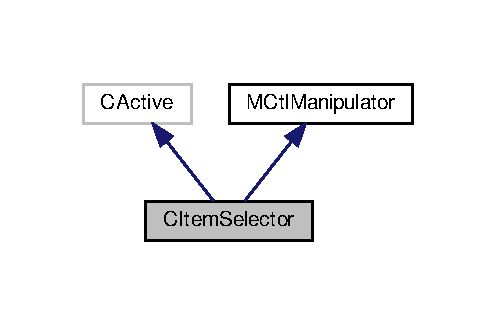
\includegraphics[width=238pt]{classCItemSelector__inherit__graph}
\end{center}
\end{figure}


Collaboration diagram for C\+Item\+Selector\+:
\nopagebreak
\begin{figure}[H]
\begin{center}
\leavevmode
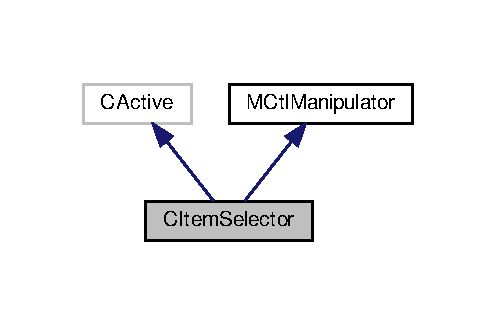
\includegraphics[width=238pt]{classCItemSelector__coll__graph}
\end{center}
\end{figure}
\subsection*{Public Member Functions}
\begin{DoxyCompactItemize}
\item 
\mbox{\Hypertarget{classCItemSelector_ae3397bf2fe1e3fcb641762ea3b78891b}\label{classCItemSelector_ae3397bf2fe1e3fcb641762ea3b78891b}} 
virtual void {\bfseries Handle\+Pointer\+EventL} (const T\+Pointer\+Event \&a\+Pointer\+Event)
\item 
\mbox{\Hypertarget{classCItemSelector_ae7ca505480c8c242821116877eb760c3}\label{classCItemSelector_ae7ca505480c8c242821116877eb760c3}} 
void {\bfseries Set\+Down\+Point} (const T\+Point \&a\+Point)
\item 
\mbox{\Hypertarget{classCItemSelector_a2241a27681ede476cf7fa1444a07a99d}\label{classCItemSelector_a2241a27681ede476cf7fa1444a07a99d}} 
void {\bfseries Start\+Select} ()
\end{DoxyCompactItemize}
\subsection*{Static Public Member Functions}
\begin{DoxyCompactItemize}
\item 
\mbox{\Hypertarget{classCItemSelector_a145c265e67ff384e294bb53e662679da}\label{classCItemSelector_a145c265e67ff384e294bb53e662679da}} 
static \hyperlink{classCItemSelector}{C\+Item\+Selector} $\ast$ \hyperlink{classCItemSelector_a145c265e67ff384e294bb53e662679da}{NewL} (\hyperlink{classCCtlColumn}{C\+Ctl\+Column} $\ast$a\+Model, C\+Video\+List\+Ctl $\ast$a\+View)
\begin{DoxyCompactList}\small\item\em \hyperlink{classCItemSelector}{C\+Item\+Selector}. \end{DoxyCompactList}\item 
\mbox{\Hypertarget{classCItemSelector_aa49db6f3acad03c14605774e4cb230ec}\label{classCItemSelector_aa49db6f3acad03c14605774e4cb230ec}} 
static \hyperlink{classCItemSelector}{C\+Item\+Selector} $\ast$ {\bfseries New\+LC} (\hyperlink{classCCtlColumn}{C\+Ctl\+Column} $\ast$a\+Model, C\+Video\+List\+Ctl $\ast$a\+View)
\end{DoxyCompactItemize}
\subsection*{Protected Types}
\begin{DoxyCompactItemize}
\item 
\mbox{\Hypertarget{classCItemSelector_a32525d4067d32c4e31c1997ae32f0011}\label{classCItemSelector_a32525d4067d32c4e31c1997ae32f0011}} 
enum {\bfseries T\+Select\+State} \{ {\bfseries K\+No\+Select}, 
{\bfseries K\+Selected}
 \}
\end{DoxyCompactItemize}
\subsection*{Protected Member Functions}
\begin{DoxyCompactItemize}
\item 
\mbox{\Hypertarget{classCItemSelector_a662af13a442c31bbafbfcea50fc58d09}\label{classCItemSelector_a662af13a442c31bbafbfcea50fc58d09}} 
{\bfseries C\+Item\+Selector} (\hyperlink{classCCtlColumn}{C\+Ctl\+Column} $\ast$a\+Model, C\+Video\+List\+Ctl $\ast$a\+View)
\item 
\mbox{\Hypertarget{classCItemSelector_aab7aa8877ccc041e2b7af3de428c17ad}\label{classCItemSelector_aab7aa8877ccc041e2b7af3de428c17ad}} 
void {\bfseries ConstructL} ()
\item 
\mbox{\Hypertarget{classCItemSelector_adc6218d680c13c924cc00ea571b6631a}\label{classCItemSelector_adc6218d680c13c924cc00ea571b6631a}} 
virtual void {\bfseries RunL} ()
\item 
\mbox{\Hypertarget{classCItemSelector_af17d0d5ca2f81d8e98a2e1d1dca1bfc0}\label{classCItemSelector_af17d0d5ca2f81d8e98a2e1d1dca1bfc0}} 
virtual void {\bfseries Do\+Cancel} ()
\item 
\mbox{\Hypertarget{classCItemSelector_ab91276eae71ea1757c47b1879728d2c1}\label{classCItemSelector_ab91276eae71ea1757c47b1879728d2c1}} 
T\+Int {\bfseries Run\+Error} (T\+Int a\+Error)
\end{DoxyCompactItemize}
\subsection*{Additional Inherited Members}


The documentation for this class was generated from the following files\+:\begin{DoxyCompactItemize}
\item 
/home/peter/work/github/\+Barba\+G\+U\+I/inc/\+Ctl/ctlmanipulator.\+h\item 
/home/peter/work/github/\+Barba\+G\+U\+I/src/\+Ctl/Ctl\+Manipulator.\+cpp\end{DoxyCompactItemize}

\hypertarget{classCMultiSelectManipulator}{}\section{C\+Multi\+Select\+Manipulator Class Reference}
\label{classCMultiSelectManipulator}\index{C\+Multi\+Select\+Manipulator@{C\+Multi\+Select\+Manipulator}}


Inheritance diagram for C\+Multi\+Select\+Manipulator\+:
\nopagebreak
\begin{figure}[H]
\begin{center}
\leavevmode
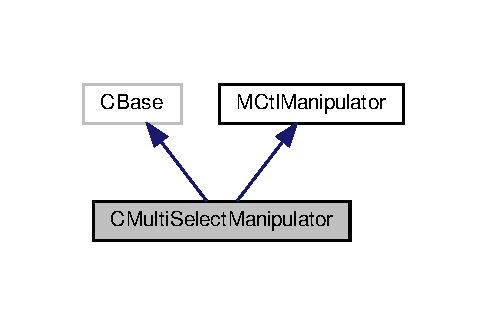
\includegraphics[width=234pt]{classCMultiSelectManipulator__inherit__graph}
\end{center}
\end{figure}


Collaboration diagram for C\+Multi\+Select\+Manipulator\+:
\nopagebreak
\begin{figure}[H]
\begin{center}
\leavevmode
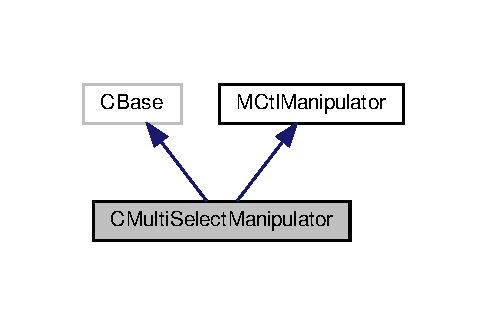
\includegraphics[width=234pt]{classCMultiSelectManipulator__coll__graph}
\end{center}
\end{figure}
\subsection*{Public Member Functions}
\begin{DoxyCompactItemize}
\item 
\mbox{\Hypertarget{classCMultiSelectManipulator_aa44d6f631c563f3676e1b45f2adea35c}\label{classCMultiSelectManipulator_aa44d6f631c563f3676e1b45f2adea35c}} 
{\bfseries C\+Multi\+Select\+Manipulator} (C\+Y\+K\+Column $\ast$a\+Model, C\+Add\+Location\+List\+Ctl $\ast$a\+View)
\item 
\mbox{\Hypertarget{classCMultiSelectManipulator_a54077536ee6578e6ced1d2ba51385a0b}\label{classCMultiSelectManipulator_a54077536ee6578e6ced1d2ba51385a0b}} 
virtual void {\bfseries Handle\+Pointer\+EventL} (const T\+Pointer\+Event \&a\+Pointer\+Event)
\end{DoxyCompactItemize}
\subsection*{Additional Inherited Members}


The documentation for this class was generated from the following file\+:\begin{DoxyCompactItemize}
\item 
/home/peter/work/github/\+Barba\+G\+U\+I/inc/\+Ctl/ctlmanipulator.\+h\end{DoxyCompactItemize}

\hypertarget{classCRowFormat}{}\section{C\+Row\+Format Class Reference}
\label{classCRowFormat}\index{C\+Row\+Format@{C\+Row\+Format}}


Inheritance diagram for C\+Row\+Format\+:
\nopagebreak
\begin{figure}[H]
\begin{center}
\leavevmode
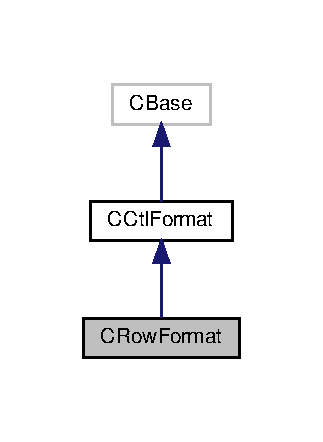
\includegraphics[width=155pt]{classCRowFormat__inherit__graph}
\end{center}
\end{figure}


Collaboration diagram for C\+Row\+Format\+:
\nopagebreak
\begin{figure}[H]
\begin{center}
\leavevmode
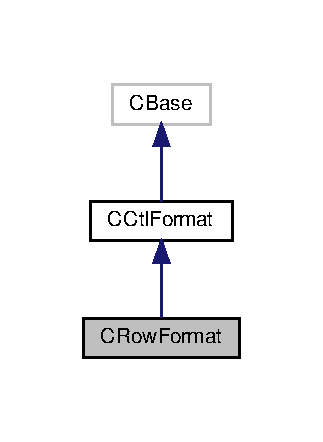
\includegraphics[width=155pt]{classCRowFormat__coll__graph}
\end{center}
\end{figure}
\subsection*{Public Member Functions}
\begin{DoxyCompactItemize}
\item 
\mbox{\Hypertarget{classCRowFormat_ae9cd333223b8df70c1302c677fba1ddf}\label{classCRowFormat_ae9cd333223b8df70c1302c677fba1ddf}} 
\hyperlink{classCRowFormat}{C\+Row\+Format} $\ast$ {\bfseries Clone} ()
\end{DoxyCompactItemize}
\subsection*{Additional Inherited Members}


The documentation for this class was generated from the following files\+:\begin{DoxyCompactItemize}
\item 
/home/peter/work/github/\+Barba\+G\+U\+I/inc/\+Ctl/Ctl\+Format.\+h\item 
/home/peter/work/github/\+Barba\+G\+U\+I/src/\+Ctl/Ctl\+Format.\+cpp\end{DoxyCompactItemize}

\hypertarget{classCRowLayout}{}\section{C\+Row\+Layout Class Reference}
\label{classCRowLayout}\index{C\+Row\+Layout@{C\+Row\+Layout}}


Inheritance diagram for C\+Row\+Layout\+:
\nopagebreak
\begin{figure}[H]
\begin{center}
\leavevmode
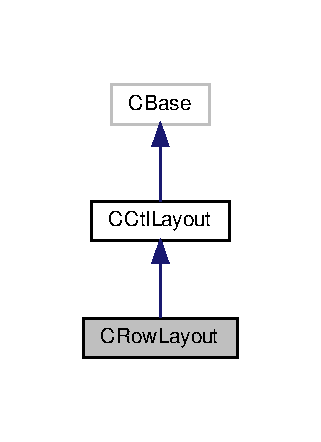
\includegraphics[width=154pt]{classCRowLayout__inherit__graph}
\end{center}
\end{figure}


Collaboration diagram for C\+Row\+Layout\+:
\nopagebreak
\begin{figure}[H]
\begin{center}
\leavevmode
\includegraphics[width=215pt]{classCRowLayout__coll__graph}
\end{center}
\end{figure}
\subsection*{Public Member Functions}
\begin{DoxyCompactItemize}
\item 
\mbox{\Hypertarget{classCRowLayout_a535248e9b72de5c552c156e22e38cb1a}\label{classCRowLayout_a535248e9b72de5c552c156e22e38cb1a}} 
void {\bfseries Set\+Format} (\hyperlink{classCRowFormat}{C\+Row\+Format} $\ast$a\+Row\+Format)
\end{DoxyCompactItemize}
\subsection*{Protected Attributes}
\begin{DoxyCompactItemize}
\item 
\mbox{\Hypertarget{classCRowLayout_a85a0046e60788ca4cd978ca353afa41c}\label{classCRowLayout_a85a0046e60788ca4cd978ca353afa41c}} 
\hyperlink{classCRowFormat}{C\+Row\+Format} $\ast$ {\bfseries i\+Format}
\end{DoxyCompactItemize}


The documentation for this class was generated from the following files\+:\begin{DoxyCompactItemize}
\item 
/home/peter/work/github/\+Barba\+G\+U\+I/inc/\+Ctl/Ctl\+Layout.\+h\item 
/home/peter/work/github/\+Barba\+G\+U\+I/src/\+Ctl/Ctl\+Layout.\+cpp\end{DoxyCompactItemize}

\hypertarget{classCScrollManipulator}{}\section{C\+Scroll\+Manipulator Class Reference}
\label{classCScrollManipulator}\index{C\+Scroll\+Manipulator@{C\+Scroll\+Manipulator}}


Inheritance diagram for C\+Scroll\+Manipulator\+:
\nopagebreak
\begin{figure}[H]
\begin{center}
\leavevmode
\includegraphics[width=234pt]{classCScrollManipulator__inherit__graph}
\end{center}
\end{figure}


Collaboration diagram for C\+Scroll\+Manipulator\+:
\nopagebreak
\begin{figure}[H]
\begin{center}
\leavevmode
\includegraphics[width=234pt]{classCScrollManipulator__coll__graph}
\end{center}
\end{figure}
\subsection*{Public Member Functions}
\begin{DoxyCompactItemize}
\item 
\hyperlink{classCScrollManipulator_a4ec182540b21abb51ccbfc8fbb04b1fe}{C\+Scroll\+Manipulator} (C\+M\+W\+Row $\ast$a\+Model, C\+Scroll\+Bar\+Ctl $\ast$a\+View)
\begin{DoxyCompactList}\small\item\em \hyperlink{classCDragManipulator}{C\+Drag\+Manipulator}. \end{DoxyCompactList}\item 
\mbox{\Hypertarget{classCScrollManipulator_a7bc1704fdc5c07ecaf76205cfaecb413}\label{classCScrollManipulator_a7bc1704fdc5c07ecaf76205cfaecb413}} 
virtual void {\bfseries Handle\+Pointer\+EventL} (const T\+Pointer\+Event \&a\+Pointer\+Event)
\end{DoxyCompactItemize}
\subsection*{Additional Inherited Members}


\subsection{Constructor \& Destructor Documentation}
\mbox{\Hypertarget{classCScrollManipulator_a4ec182540b21abb51ccbfc8fbb04b1fe}\label{classCScrollManipulator_a4ec182540b21abb51ccbfc8fbb04b1fe}} 
\index{C\+Scroll\+Manipulator@{C\+Scroll\+Manipulator}!C\+Scroll\+Manipulator@{C\+Scroll\+Manipulator}}
\index{C\+Scroll\+Manipulator@{C\+Scroll\+Manipulator}!C\+Scroll\+Manipulator@{C\+Scroll\+Manipulator}}
\subsubsection{\texorpdfstring{C\+Scroll\+Manipulator()}{CScrollManipulator()}}
{\footnotesize\ttfamily C\+Scroll\+Manipulator\+::\+C\+Scroll\+Manipulator (\begin{DoxyParamCaption}\item[{C\+M\+W\+Row $\ast$}]{a\+Model,  }\item[{C\+Scroll\+Bar\+Ctl $\ast$}]{a\+View }\end{DoxyParamCaption})}



\hyperlink{classCDragManipulator}{C\+Drag\+Manipulator}. 

\hyperlink{classCScrollManipulator}{C\+Scroll\+Manipulator} 

The documentation for this class was generated from the following files\+:\begin{DoxyCompactItemize}
\item 
/home/peter/work/github/\+Barba\+G\+U\+I/inc/\+Ctl/ctlmanipulator.\+h\item 
/home/peter/work/github/\+Barba\+G\+U\+I/src/\+Ctl/Ctl\+Manipulator.\+cpp\end{DoxyCompactItemize}

\hypertarget{classMCtlListBoxObserver}{}\section{M\+Ctl\+List\+Box\+Observer Class Reference}
\label{classMCtlListBoxObserver}\index{M\+Ctl\+List\+Box\+Observer@{M\+Ctl\+List\+Box\+Observer}}
\subsection*{Public Types}
\begin{DoxyCompactItemize}
\item 
enum \hyperlink{classMCtlListBoxObserver_ab9551a8e542c692650a2d4254418597f}{T\+Ctl\+List\+Box\+Event} \{ \newline
\hyperlink{classMCtlListBoxObserver_ab9551a8e542c692650a2d4254418597fa4ba478a28f09b91b393e893ac08139c1}{E\+Event\+Item\+Tapped}, 
\hyperlink{classMCtlListBoxObserver_ab9551a8e542c692650a2d4254418597fabc92b03e912556c47089bd5e91735863}{E\+Event\+Item\+Highlighted}, 
\hyperlink{classMCtlListBoxObserver_ab9551a8e542c692650a2d4254418597fab6706ed10da78be090cf70af8d680ffc}{E\+Event\+Item\+Confirmed}, 
\hyperlink{classMCtlListBoxObserver_ab9551a8e542c692650a2d4254418597fa95724c42e1f845e1c36dfcb3d0ec9f37}{E\+Event\+Selection\+Changed}, 
\newline
\hyperlink{classMCtlListBoxObserver_ab9551a8e542c692650a2d4254418597fa8421c10105c6b882cb17a1f3166f834f}{E\+Event\+Match\+Buffer\+Changed}, 
\hyperlink{classMCtlListBoxObserver_ab9551a8e542c692650a2d4254418597faa21a7a3c75c3659a36b89307e291a03a}{E\+Event\+Top\+Reached}, 
\hyperlink{classMCtlListBoxObserver_ab9551a8e542c692650a2d4254418597fa43824f6c25215002bdef837408b5bc73}{E\+Event\+Bottom\+Reached}, 
\hyperlink{classMCtlListBoxObserver_ab9551a8e542c692650a2d4254418597fa035e3f0c21ddc1616b3761ef1f3f5ac7}{E\+Event\+Empty\+List\+Box\+Actioned}, 
\newline
\hyperlink{classMCtlListBoxObserver_ab9551a8e542c692650a2d4254418597fa0b2b5240900e68d90e4fa1b12cb3e3bf}{E\+Event\+Highlight\+Moved}, 
\hyperlink{classMCtlListBoxObserver_ab9551a8e542c692650a2d4254418597faf2bb42155bddf80e5a39b304fe326498}{E\+Event\+Slot\+Index\+Changed}, 
\hyperlink{classMCtlListBoxObserver_ab9551a8e542c692650a2d4254418597faee24f3770660c68409bd84bfa6697045}{E\+Event\+Dimmed\+Item\+Confirmed\+Attempt}, 
\hyperlink{classMCtlListBoxObserver_ab9551a8e542c692650a2d4254418597fa1355ee232ee0fd81b51542c9623d2635}{E\+Event\+Match\+Buffer\+Full}, 
\newline
\hyperlink{classMCtlListBoxObserver_ab9551a8e542c692650a2d4254418597fadf0d22a23099fd63cf17bbe65ea663db}{E\+Event\+Custom\+Start} = 0x1000
 \}
\end{DoxyCompactItemize}
\subsection*{Public Member Functions}
\begin{DoxyCompactItemize}
\item 
virtual void \hyperlink{classMCtlListBoxObserver_a346b02a3826ff1f15a61082e38dab958}{Handle\+List\+Box\+EventL} (\hyperlink{classCCtlListBox}{C\+Ctl\+List\+Box} $\ast$a\+List\+Box, \hyperlink{classMCtlListBoxObserver_ab9551a8e542c692650a2d4254418597f}{T\+Ctl\+List\+Box\+Event} a\+Event\+Type, T\+Int a\+Item\+Index, T\+Int a\+Slot\+Id)=0
\end{DoxyCompactItemize}


\subsection{Member Enumeration Documentation}
\mbox{\Hypertarget{classMCtlListBoxObserver_ab9551a8e542c692650a2d4254418597f}\label{classMCtlListBoxObserver_ab9551a8e542c692650a2d4254418597f}} 
\index{M\+Ctl\+List\+Box\+Observer@{M\+Ctl\+List\+Box\+Observer}!T\+Ctl\+List\+Box\+Event@{T\+Ctl\+List\+Box\+Event}}
\index{T\+Ctl\+List\+Box\+Event@{T\+Ctl\+List\+Box\+Event}!M\+Ctl\+List\+Box\+Observer@{M\+Ctl\+List\+Box\+Observer}}
\subsubsection{\texorpdfstring{T\+Ctl\+List\+Box\+Event}{TCtlListBoxEvent}}
{\footnotesize\ttfamily enum \hyperlink{classMCtlListBoxObserver_ab9551a8e542c692650a2d4254418597f}{M\+Ctl\+List\+Box\+Observer\+::\+T\+Ctl\+List\+Box\+Event}}

List box event codes. \begin{DoxyEnumFields}{Enumerator}
\raisebox{\heightof{T}}[0pt][0pt]{\index{E\+Event\+Item\+Tapped@{E\+Event\+Item\+Tapped}!M\+Ctl\+List\+Box\+Observer@{M\+Ctl\+List\+Box\+Observer}}\index{M\+Ctl\+List\+Box\+Observer@{M\+Ctl\+List\+Box\+Observer}!E\+Event\+Item\+Tapped@{E\+Event\+Item\+Tapped}}}\mbox{\Hypertarget{classMCtlListBoxObserver_ab9551a8e542c692650a2d4254418597fa4ba478a28f09b91b393e893ac08139c1}\label{classMCtlListBoxObserver_ab9551a8e542c692650a2d4254418597fa4ba478a28f09b91b393e893ac08139c1}} 
E\+Event\+Item\+Tapped&This event is reported when an item is tapped, and denotes a user action on an item. This event is reported somewhat differently for items having a highlight layout and those that does not.

When an item, having only a normal layout, is tapped on this event is triggered.

An item that has a highlight layout, needs to be highlighted and then tapped for this event to be reported.

The observer is allowed to change the state of the List Box and its components when receiving this event. \\
\hline

\raisebox{\heightof{T}}[0pt][0pt]{\index{E\+Event\+Item\+Highlighted@{E\+Event\+Item\+Highlighted}!M\+Ctl\+List\+Box\+Observer@{M\+Ctl\+List\+Box\+Observer}}\index{M\+Ctl\+List\+Box\+Observer@{M\+Ctl\+List\+Box\+Observer}!E\+Event\+Item\+Highlighted@{E\+Event\+Item\+Highlighted}}}\mbox{\Hypertarget{classMCtlListBoxObserver_ab9551a8e542c692650a2d4254418597fabc92b03e912556c47089bd5e91735863}\label{classMCtlListBoxObserver_ab9551a8e542c692650a2d4254418597fabc92b03e912556c47089bd5e91735863}} 
E\+Event\+Item\+Highlighted&This event is reported when a item having a highlight layout but not currently highlighted, is tapped. In this case a {\ttfamily E\+Event\+Highlight\+Moved} event will be reported first, followed by this event. Can be used as a way to distinguish between pen or key cause of highlight moved.

The observer is allowed to change the state of the List Box and its components when receiving this event. \\
\hline

\raisebox{\heightof{T}}[0pt][0pt]{\index{E\+Event\+Item\+Confirmed@{E\+Event\+Item\+Confirmed}!M\+Ctl\+List\+Box\+Observer@{M\+Ctl\+List\+Box\+Observer}}\index{M\+Ctl\+List\+Box\+Observer@{M\+Ctl\+List\+Box\+Observer}!E\+Event\+Item\+Confirmed@{E\+Event\+Item\+Confirmed}}}\mbox{\Hypertarget{classMCtlListBoxObserver_ab9551a8e542c692650a2d4254418597fab6706ed10da78be090cf70af8d680ffc}\label{classMCtlListBoxObserver_ab9551a8e542c692650a2d4254418597fab6706ed10da78be090cf70af8d680ffc}} 
E\+Event\+Item\+Confirmed&Item confirm event. When an item is selected using select soft key.

The observer is allowed to change the state of the List Box and its components when receiving this event. \\
\hline

\raisebox{\heightof{T}}[0pt][0pt]{\index{E\+Event\+Selection\+Changed@{E\+Event\+Selection\+Changed}!M\+Ctl\+List\+Box\+Observer@{M\+Ctl\+List\+Box\+Observer}}\index{M\+Ctl\+List\+Box\+Observer@{M\+Ctl\+List\+Box\+Observer}!E\+Event\+Selection\+Changed@{E\+Event\+Selection\+Changed}}}\mbox{\Hypertarget{classMCtlListBoxObserver_ab9551a8e542c692650a2d4254418597fa95724c42e1f845e1c36dfcb3d0ec9f37}\label{classMCtlListBoxObserver_ab9551a8e542c692650a2d4254418597fa95724c42e1f845e1c36dfcb3d0ec9f37}} 
E\+Event\+Selection\+Changed&An item has been selected or deselected in a multiple slect enabled List Box. If more then one item is affected the event will be reported with index parameters having value E\+Qik\+List\+Box\+Param\+Not\+Applicable.

The observer must not alter the state of any List Box components when receiving this event. \\
\hline

\raisebox{\heightof{T}}[0pt][0pt]{\index{E\+Event\+Match\+Buffer\+Changed@{E\+Event\+Match\+Buffer\+Changed}!M\+Ctl\+List\+Box\+Observer@{M\+Ctl\+List\+Box\+Observer}}\index{M\+Ctl\+List\+Box\+Observer@{M\+Ctl\+List\+Box\+Observer}!E\+Event\+Match\+Buffer\+Changed@{E\+Event\+Match\+Buffer\+Changed}}}\mbox{\Hypertarget{classMCtlListBoxObserver_ab9551a8e542c692650a2d4254418597fa8421c10105c6b882cb17a1f3166f834f}\label{classMCtlListBoxObserver_ab9551a8e542c692650a2d4254418597fa8421c10105c6b882cb17a1f3166f834f}} 
E\+Event\+Match\+Buffer\+Changed&The buffer that holds the characters that has currently been matched, has changed.

The observer must not alter the state of any List Box components when receiving this event. \\
\hline

\raisebox{\heightof{T}}[0pt][0pt]{\index{E\+Event\+Top\+Reached@{E\+Event\+Top\+Reached}!M\+Ctl\+List\+Box\+Observer@{M\+Ctl\+List\+Box\+Observer}}\index{M\+Ctl\+List\+Box\+Observer@{M\+Ctl\+List\+Box\+Observer}!E\+Event\+Top\+Reached@{E\+Event\+Top\+Reached}}}\mbox{\Hypertarget{classMCtlListBoxObserver_ab9551a8e542c692650a2d4254418597faa21a7a3c75c3659a36b89307e291a03a}\label{classMCtlListBoxObserver_ab9551a8e542c692650a2d4254418597faa21a7a3c75c3659a36b89307e291a03a}} 
E\+Event\+Top\+Reached&The top of the list has been reached. Event generated when standing on top item and trying to go up.

The observer must not alter the state of any List Box components when receiving this event. \\
\hline

\raisebox{\heightof{T}}[0pt][0pt]{\index{E\+Event\+Bottom\+Reached@{E\+Event\+Bottom\+Reached}!M\+Ctl\+List\+Box\+Observer@{M\+Ctl\+List\+Box\+Observer}}\index{M\+Ctl\+List\+Box\+Observer@{M\+Ctl\+List\+Box\+Observer}!E\+Event\+Bottom\+Reached@{E\+Event\+Bottom\+Reached}}}\mbox{\Hypertarget{classMCtlListBoxObserver_ab9551a8e542c692650a2d4254418597fa43824f6c25215002bdef837408b5bc73}\label{classMCtlListBoxObserver_ab9551a8e542c692650a2d4254418597fa43824f6c25215002bdef837408b5bc73}} 
E\+Event\+Bottom\+Reached&The bottom of the list has been reached. Event generated when standing on last item and trying to go down.

The observer must not alter the state of any List Box components when receiving this event. \\
\hline

\raisebox{\heightof{T}}[0pt][0pt]{\index{E\+Event\+Empty\+List\+Box\+Actioned@{E\+Event\+Empty\+List\+Box\+Actioned}!M\+Ctl\+List\+Box\+Observer@{M\+Ctl\+List\+Box\+Observer}}\index{M\+Ctl\+List\+Box\+Observer@{M\+Ctl\+List\+Box\+Observer}!E\+Event\+Empty\+List\+Box\+Actioned@{E\+Event\+Empty\+List\+Box\+Actioned}}}\mbox{\Hypertarget{classMCtlListBoxObserver_ab9551a8e542c692650a2d4254418597fa035e3f0c21ddc1616b3761ef1f3f5ac7}\label{classMCtlListBoxObserver_ab9551a8e542c692650a2d4254418597fa035e3f0c21ddc1616b3761ef1f3f5ac7}} 
E\+Event\+Empty\+List\+Box\+Actioned&A tap in an empty List Box generates this event.

The observer is allowed to change the state of the List Box and its components when receiving this event. \\
\hline

\raisebox{\heightof{T}}[0pt][0pt]{\index{E\+Event\+Highlight\+Moved@{E\+Event\+Highlight\+Moved}!M\+Ctl\+List\+Box\+Observer@{M\+Ctl\+List\+Box\+Observer}}\index{M\+Ctl\+List\+Box\+Observer@{M\+Ctl\+List\+Box\+Observer}!E\+Event\+Highlight\+Moved@{E\+Event\+Highlight\+Moved}}}\mbox{\Hypertarget{classMCtlListBoxObserver_ab9551a8e542c692650a2d4254418597fa0b2b5240900e68d90e4fa1b12cb3e3bf}\label{classMCtlListBoxObserver_ab9551a8e542c692650a2d4254418597fa0b2b5240900e68d90e4fa1b12cb3e3bf}} 
E\+Event\+Highlight\+Moved&The highlight has moved.

The observer must not alter the state of any List Box components when receiving this event. \\
\hline

\raisebox{\heightof{T}}[0pt][0pt]{\index{E\+Event\+Slot\+Index\+Changed@{E\+Event\+Slot\+Index\+Changed}!M\+Ctl\+List\+Box\+Observer@{M\+Ctl\+List\+Box\+Observer}}\index{M\+Ctl\+List\+Box\+Observer@{M\+Ctl\+List\+Box\+Observer}!E\+Event\+Slot\+Index\+Changed@{E\+Event\+Slot\+Index\+Changed}}}\mbox{\Hypertarget{classMCtlListBoxObserver_ab9551a8e542c692650a2d4254418597faf2bb42155bddf80e5a39b304fe326498}\label{classMCtlListBoxObserver_ab9551a8e542c692650a2d4254418597faf2bb42155bddf80e5a39b304fe326498}} 
E\+Event\+Slot\+Index\+Changed&The index on the slot has changed.

The observer must not alter the state of any List Box components when receiving this event. \\
\hline

\raisebox{\heightof{T}}[0pt][0pt]{\index{E\+Event\+Dimmed\+Item\+Confirmed\+Attempt@{E\+Event\+Dimmed\+Item\+Confirmed\+Attempt}!M\+Ctl\+List\+Box\+Observer@{M\+Ctl\+List\+Box\+Observer}}\index{M\+Ctl\+List\+Box\+Observer@{M\+Ctl\+List\+Box\+Observer}!E\+Event\+Dimmed\+Item\+Confirmed\+Attempt@{E\+Event\+Dimmed\+Item\+Confirmed\+Attempt}}}\mbox{\Hypertarget{classMCtlListBoxObserver_ab9551a8e542c692650a2d4254418597faee24f3770660c68409bd84bfa6697045}\label{classMCtlListBoxObserver_ab9551a8e542c692650a2d4254418597faee24f3770660c68409bd84bfa6697045}} 
E\+Event\+Dimmed\+Item\+Confirmed\+Attempt&An attempt to confirm a dimmed item has been made.

The observer is allowed to change the state of the List Box and its components when receiving this event. \\
\hline

\raisebox{\heightof{T}}[0pt][0pt]{\index{E\+Event\+Match\+Buffer\+Full@{E\+Event\+Match\+Buffer\+Full}!M\+Ctl\+List\+Box\+Observer@{M\+Ctl\+List\+Box\+Observer}}\index{M\+Ctl\+List\+Box\+Observer@{M\+Ctl\+List\+Box\+Observer}!E\+Event\+Match\+Buffer\+Full@{E\+Event\+Match\+Buffer\+Full}}}\mbox{\Hypertarget{classMCtlListBoxObserver_ab9551a8e542c692650a2d4254418597fa1355ee232ee0fd81b51542c9623d2635}\label{classMCtlListBoxObserver_ab9551a8e542c692650a2d4254418597fa1355ee232ee0fd81b51542c9623d2635}} 
E\+Event\+Match\+Buffer\+Full&The incremental match buffer is full, the maximum number of characters to match on has been reached.

The observer must not alter the state of any List Box components when receiving this event. \\
\hline

\raisebox{\heightof{T}}[0pt][0pt]{\index{E\+Event\+Custom\+Start@{E\+Event\+Custom\+Start}!M\+Ctl\+List\+Box\+Observer@{M\+Ctl\+List\+Box\+Observer}}\index{M\+Ctl\+List\+Box\+Observer@{M\+Ctl\+List\+Box\+Observer}!E\+Event\+Custom\+Start@{E\+Event\+Custom\+Start}}}\mbox{\Hypertarget{classMCtlListBoxObserver_ab9551a8e542c692650a2d4254418597fadf0d22a23099fd63cf17bbe65ea663db}\label{classMCtlListBoxObserver_ab9551a8e542c692650a2d4254418597fadf0d22a23099fd63cf17bbe65ea663db}} 
E\+Event\+Custom\+Start&Custom events section start.

The observer must not alter the state of any List Box components when receiving this event. \\
\hline

\end{DoxyEnumFields}


\subsection{Member Function Documentation}
\mbox{\Hypertarget{classMCtlListBoxObserver_a346b02a3826ff1f15a61082e38dab958}\label{classMCtlListBoxObserver_a346b02a3826ff1f15a61082e38dab958}} 
\index{M\+Ctl\+List\+Box\+Observer@{M\+Ctl\+List\+Box\+Observer}!Handle\+List\+Box\+EventL@{Handle\+List\+Box\+EventL}}
\index{Handle\+List\+Box\+EventL@{Handle\+List\+Box\+EventL}!M\+Ctl\+List\+Box\+Observer@{M\+Ctl\+List\+Box\+Observer}}
\subsubsection{\texorpdfstring{Handle\+List\+Box\+Event\+L()}{HandleListBoxEventL()}}
{\footnotesize\ttfamily virtual void M\+Ctl\+List\+Box\+Observer\+::\+Handle\+List\+Box\+EventL (\begin{DoxyParamCaption}\item[{\hyperlink{classCCtlListBox}{C\+Ctl\+List\+Box} $\ast$}]{a\+List\+Box,  }\item[{\hyperlink{classMCtlListBoxObserver_ab9551a8e542c692650a2d4254418597f}{T\+Ctl\+List\+Box\+Event}}]{a\+Event\+Type,  }\item[{T\+Int}]{a\+Item\+Index,  }\item[{T\+Int}]{a\+Slot\+Id }\end{DoxyParamCaption})\hspace{0.3cm}{\ttfamily [pure virtual]}}

Handles list box events.

This pure virtual function is invoked by {\ttfamily C\+Qik\+List\+Box} to notify the observer of list box events.

The List Box observer must never alter the state of the List Box or any of its components while in between a M\+Qik\+List\+Box\+Model\+::\+Model\+Begin\+Update\+LC and a M\+Qik\+List\+Box\+Model\+::\+Model\+End\+UpdateL call. Further more each event either allows or forbids altering of the List Box and its components upon receving the particular event, see {\ttfamily T\+Qik\+List\+Box\+Event} for further information on this.


\begin{DoxyParams}{Parameters}
{\em a\+List\+Box} & The originating list box. \\
\hline
{\em a\+Event\+Type} & A code for the event. Further information may be obtained by accessing the list box itself. \\
\hline
{\em a\+Item\+Index} & The item index, if applicable, else E\+Qik\+List\+Box\+Param\+Not\+Applicable. \\
\hline
{\em a\+Slot\+Id} & The item slot id the event was generated in, if applicable, else E\+Qik\+List\+Box\+Param\+Not\+Applicable. \\
\hline
\end{DoxyParams}


The documentation for this class was generated from the following file\+:\begin{DoxyCompactItemize}
\item 
/home/peter/work/github/\+Barba\+G\+U\+I/inc/\+Ctl/Ctl\+List\+Box\+Observer.\+h\end{DoxyCompactItemize}

\hypertarget{classMCtlManipulator}{}\section{M\+Ctl\+Manipulator Class Reference}
\label{classMCtlManipulator}\index{M\+Ctl\+Manipulator@{M\+Ctl\+Manipulator}}


Inheritance diagram for M\+Ctl\+Manipulator\+:
\nopagebreak
\begin{figure}[H]
\begin{center}
\leavevmode
\includegraphics[width=327pt]{classMCtlManipulator__inherit__graph}
\end{center}
\end{figure}
\subsection*{Public Member Functions}
\begin{DoxyCompactItemize}
\item 
\mbox{\Hypertarget{classMCtlManipulator_a5e955bea06960e9f44db70047bfce4f0}\label{classMCtlManipulator_a5e955bea06960e9f44db70047bfce4f0}} 
T\+Bool {\bfseries Is\+Active} ()
\item 
\mbox{\Hypertarget{classMCtlManipulator_aaf3d6b58180c46e34532140606db97d4}\label{classMCtlManipulator_aaf3d6b58180c46e34532140606db97d4}} 
\hyperlink{classMCtlManipulator_aaf3d6b58180c46e34532140606db97d4}{M\+Ctl\+Manipulator} ()
\begin{DoxyCompactList}\small\item\em \hyperlink{classMCtlManipulator}{M\+Ctl\+Manipulator}. \end{DoxyCompactList}\item 
\mbox{\Hypertarget{classMCtlManipulator_a7ce0be9715912a544ee738a63f1e9e08}\label{classMCtlManipulator_a7ce0be9715912a544ee738a63f1e9e08}} 
virtual void {\bfseries Handle\+Pointer\+EventL} (const T\+Pointer\+Event \&a\+Pointer\+Event)
\item 
\mbox{\Hypertarget{classMCtlManipulator_aa25d6b77b3f0b2ef8342f714d9795fbf}\label{classMCtlManipulator_aa25d6b77b3f0b2ef8342f714d9795fbf}} 
virtual void {\bfseries Draw} (C\+Window\+Gc \&gc) const
\end{DoxyCompactItemize}
\subsection*{Protected Attributes}
\begin{DoxyCompactItemize}
\item 
\mbox{\Hypertarget{classMCtlManipulator_a68584897df4007cfe1ae602ae671198c}\label{classMCtlManipulator_a68584897df4007cfe1ae602ae671198c}} 
T\+Bool {\bfseries i\+Is\+Active}
\end{DoxyCompactItemize}


The documentation for this class was generated from the following files\+:\begin{DoxyCompactItemize}
\item 
/home/peter/work/github/\+Barba\+G\+U\+I/inc/\+Ctl/ctlmanipulator.\+h\item 
/home/peter/work/github/\+Barba\+G\+U\+I/src/\+Ctl/Ctl\+Manipulator.\+cpp\end{DoxyCompactItemize}

\hypertarget{classMManipulatedView}{}\section{M\+Manipulated\+View Class Reference}
\label{classMManipulatedView}\index{M\+Manipulated\+View@{M\+Manipulated\+View}}
\subsection*{Public Member Functions}
\begin{DoxyCompactItemize}
\item 
\mbox{\Hypertarget{classMManipulatedView_a66605d81c25a0f577fd2ae6cf044a7a1}\label{classMManipulatedView_a66605d81c25a0f577fd2ae6cf044a7a1}} 
virtual void {\bfseries Draw\+Deferred} () const
\item 
\mbox{\Hypertarget{classMManipulatedView_a00807a16ce123251bd3b19ae62dc9d14}\label{classMManipulatedView_a00807a16ce123251bd3b19ae62dc9d14}} 
virtual void {\bfseries Reverse\+Select\+State} (C\+M\+W\+Row $\ast$)
\item 
\mbox{\Hypertarget{classMManipulatedView_a9b64587f5b9bf82a1987d7f62ccb0bcd}\label{classMManipulatedView_a9b64587f5b9bf82a1987d7f62ccb0bcd}} 
virtual void {\bfseries Refresh\+Select\+State} (C\+M\+W\+Row $\ast$a\+Row)
\end{DoxyCompactItemize}


The documentation for this class was generated from the following file\+:\begin{DoxyCompactItemize}
\item 
/home/peter/work/github/\+Barba\+G\+U\+I/inc/\+Ctl/ctlmanipulator.\+h\end{DoxyCompactItemize}

%--- End generated contents ---

% Index
\backmatter
\newpage
\phantomsection
\clearemptydoublepage
\addcontentsline{toc}{chapter}{Index}
\printindex

\end{document}
